\documentclass[a4paper,12pt]{book}
\usepackage[utf8]{inputenc}
\usepackage{graphicx}
\usepackage{array}
\usepackage{amsmath} 
\usepackage{amsthm}
\usepackage{tcolorbox}
\usepackage{pgfplots}
\usepackage{multicol}
\usepackage{pgfplots}
\usepackage{cancel}
\usepackage{soul}
\usepackage{amssymb}
\usepackage{mathtools}


\newcommand\ddfrac[2]{\frac{\displaystyle #1}{\displaystyle #2}}

\newcommand{\verteq}{\rotatebox{90}{$\,=$}}
\newcommand{\equalto}[2]{\underset{\scriptstyle\overset{\mkern4mu\verteq}{#2}}{#1}}

\begin{document}
	
\newcommand{\formule}[2]{
	\par\medskip\noindent%
	\begin{tabular*}{\linewidth}{@{}
			>{\centering$\displaystyle}p{\dimexpr0.24\linewidth-2\tabcolsep}<{$} % <---
			m{\dimexpr0.56\linewidth-2\tabcolsep}
			@{}}
		#1 & #2  
	\end{tabular*}\par\medskip\noindent}


\author{Simone Fabbri}
\title{Appunti di Modelli Probabilistici}
\date{Aggiornato al \today}

\frontmatter
\maketitle

\section*{Disclaimer}
\hl{Non mi assumo responsabilita' per inesattezze o errori dei contenuti.} Se anzi ne trovaste, sarei infinitamente grato se li segnalaste per mail a \\ \texttt{simone.fabbri8 at studio.unibo.it} oppure tramite la pagina del repository \texttt{https://github.com/fabbrus97/mod\_prob}. 

\tableofcontents

\mainmatter
%\chapter{The First Chapter}
%\chapter{The Second Chapter}
\chapter{Introduzione}
\section{Notazione}
\paragraph{Evento} quantità che vale 1 se si verifica, 0 se non si verifica. 

Data questa premessa, possiamo far corrispondere le operazioni insiemistiche sugli eventi a operazioni sui numeri $ E $ ed $ F $; possiamo associare a questi eventi una variabile aleatoria (che può assumere valori compresi tra 0 e 1):

\begin{center}
	\begin{tabular}{ p{4cm}|p{9cm} }	
		\hline
		\\
		\textbf{Unione} $ E \bigcup F $ & massimo tra E ed F, vale 1 se almeno un evento di verifica; somma logica \\
		\hline
		\\
		\textbf{Intersezione} $ E \cap F $ & è il minimo tra i due eventi; è detto anche prodotto logico \\
		\hline
		\\
		\textbf{Complementazione} $\widetilde{E} = 1 - E$ & si verifica se E non si verifica \\
		\hline
	\end{tabular}
\end{center}

\paragraph{Attesa (expectation)} concetto associato ai ??? aleatori.  
%TODO 
Indicheremo con lo stesso simbolo sia l'attesa, sia la probabilità: $$P(E) \qquad \qquad \qquad P(X)$$ con $E$ un evento, $ X $ indica una variabile aleatoria. 

Possiamo considerare un evento come una variabile aleatoria che può assumere solo i valori 0 e 1. 

\chapter{Passeggiate aleatorie}
\section{Schema di Bernoulli}
Effettuiamo prove indipendenti che possono dare due risultati sempre nelle stesse condizioni e che non si influenzano tra loro. 

Supponiamo di avere una successione di eventi infiniti (\textbf{nota bene} negli esempi useremo un numero finito).
Tutti gli eventi hanno la stessa probabilità:
$$P(E_i) = p$$
Quando si parla di schema di Bernoulli, bisogna specificare p.

Come formalizziamo l'altra ipotesi, ovvero che gli eventi siano indipendenti?
$$P (F_1, ..., F_i ) = p^k(1-p)^{n-k}$$
con $ F_i = E_i $ oppure $ F_i = \widetilde{E}_i $, $ p $ la costante associata allo schema di Bernoulli, $ k $ numero di volte in cui appare l'evento: in alcuni $ F_i $ infatti apparirà l'evento, in altri il complementare; $ n-k $ quindi è il numero di volte in cui appare l'evento complementare.

\section{Passeggiata aleatoria}
È il primo esempio che incontriamo di un \textbf{processo stocastico}. 

Un processo stocastico è una successione di variabili aleatorie che dipende da un parametro, tipicamente il tempo. Il tempo nello specifico viene considerato a valori discreti. 

Esempio: una particella che a t=0 si trova nel punto 0, ad ogni istante fa un passo a destra con probabilità $ p $ oppure a sinistra con probabilità $ 1-p $. 

La probabilità di andare a destra (sinistra) è costante, e le probabilità di girare in una direzione sono indipendenti. 

Dati $ E_1, E_2, E_3... $ definiamo
$$x_i = 2E_i - 1$$

\begin{align*}
	se \qquad & E_i = 1 \Rightarrow x=1, \\
	se \qquad & E_i = 0 \Rightarrow x=-1
\end{align*}

$ 1, -1 $ rappresentano lo spostamento nella nostra passeggiata aleatoria. 
\\
\\
Chiamiamo $ S_n $ lo spostamento, che rappresenta la posizione al tempo $ n $:
\begin{center}
\begin{align*}
	S_n & = \sum_{i=1}^{n} x_i \\
	& = 2(\sum_{i=1}^{n}E_i)-n \qquad \qquad \text{ detto } z_n = \sum_{i=1}^{n} E_i \\
	& = 2z_n - n
\end{align*}
\end{center}

Qual è la probabilità che ci può interessare? Dato un istante n, possiamo ad esempio chiederci la probabilità che la particella si trovi in una certa posizione (ovvero $ S_n = x $):
$$ P(S_n = x) $$

Che possiamo riscrivere come:
$$ P(2z_n - n = x) = P(z_n = \frac{n+x}{2})$$


\begin{tcolorbox}
	\paragraph{Distribuzione binomiale} disribuzione del numero di successi, quando facciamo delle prove indipendenti. 
	
	Distribuzione binomiale di parametri n e p:
	$$P(u - k) = \binom{n}{k} \cdot p^k(1-p)^{n-k}$$
	con n il numero delle prove e p la probabilità di successo. 
\end{tcolorbox}


$\ddfrac{n+x}{2}$ deve essere un numero intero, quindi $ n+x $ deve essere pari; quindi se $ n $ è pari (il tempo è pari) $ x $ deve essere pari, la particella cioè deve essere in una posizione pari:

$$\Rightarrow P(z_n = \frac{n+x}{2}) = ???$$
%TODO

La passeggiata aleatoria è definita su numeri interi, sarebbe graficamente cioè una successione di punti, ma si può visualizzare come una linea spezzata unendo i punti. 

\paragraph{Passeggiata aleatoria simmetrica} è un caso interessante di passeggiata aleatoria, dove $ p = \frac{1}{2} $: la probabilità di andare a sinistra o a destra è uguale. 

Nel grafico, quando aumento di 1 la linea sale di 1; quando x vale -1, scendo. 

\begin{tikzpicture}
	\begin{axis}[axis lines=middle, axis equal]
	\addplot coordinates{(0,0)  (1,1)};	
	\addplot coordinates{(1,1)  (2,0)};	
	\addplot coordinates{(2,0)  (3,1)};
	\addplot coordinates{(3,1)  (4,0)};	
	\addplot coordinates{(4,0)  (5,1)};	
	\end{axis}
\end{tikzpicture}

Vogliamo calcolare la probabilità di un evento che si riferisce al cammino. Dobbiamo fare la somma di tutti i casi elementari dell'evento. Sia $ A $ un evento:

$$A = \frac{\text{numero dei casi elementari}}{2^n}$$

In questo caso quindi ci riduciamo ad un \textit{problema combinatorio} (contare i casi elementari). Possiamo quindi calcolare la probabilità in modo combinatorio. 

\section{Problema del ballottaggio}
Supponiamo che ci sia un'elezione con 2 candidati. L'urna dei voti conterrà voti a favore del candidato A oppure del candidato B; Sia $ n $ il numero dei voti, e sia $ a $ il numero dei voti per $ A $ e $ b $ il numero dei voti per $ B $.  Supponiamo ancora $ a > b $. 

Mentre estraiamo le varie schede, possiamo disegnare una passeggiata aleatoria: estraendo un voto per $ A $ facciamo un passo a destra, per $ B $ a sinistra:
\begin{center}
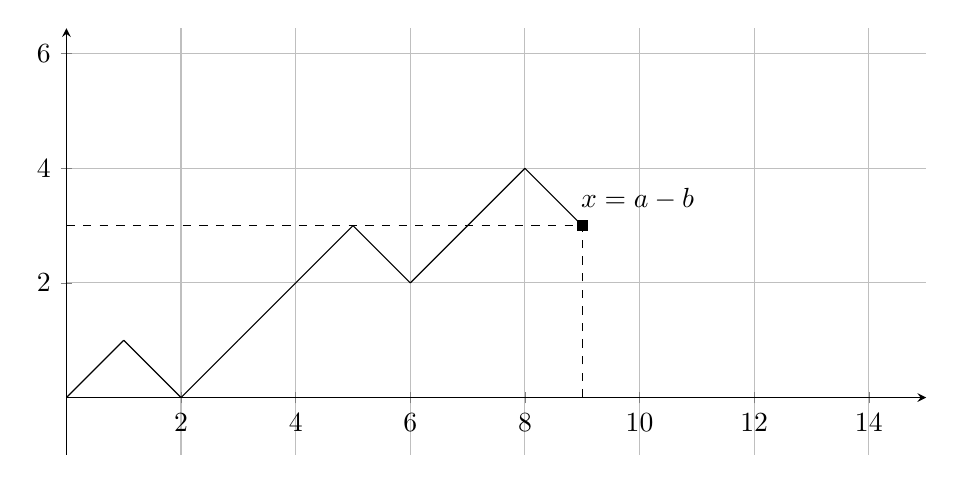
\begin{tikzpicture}
\begin{axis}[axis lines=middle, axis equal, grid=both, xmax=15, width=12.5cm, ymin=-1, height=7cm]
\addplot [color=black] coordinates{(0,0)  (1,1)};	
\addplot [color=black] coordinates{(1,1)  (2,0)};	
\addplot [color=black] coordinates{(2,0)  (3,1)};
\addplot [color=black] coordinates{(3,1)  (4,2)};
\addplot [color=black] coordinates{(4,2)  (5,3)};
\addplot [color=black] coordinates{(5,3)  (6,2)};
\addplot [color=black] coordinates{(6,2)  (7,3)};
\addplot [color=black] coordinates{(7,3)  (8,4)};
\addplot [color=black] coordinates{(8,4)  (9,3)};	
\node[label={$ \qquad\qquad x = a - b $}, fill,inner sep=2pt] at (axis cs:9,3) {};
\addplot [dashed] coordinates{(0,3) (9,3)};
\addplot [dashed] coordinates{(9,0) (9,3)};
\end{axis}
\end{tikzpicture}
\end{center}

Dove sarà la linea spezzata quando avremo estratto tutte le schede? Quando avremo fatto $ a $ passi a destra e $ b $ a sinistra, la posizione sarà $ a-b $. 

Ci chiediamo ora: qual è la probabilità che \textbf{A} sia sempre in vantaggio?

In questo caso non abbiamo tutti i cammini con probabilità uguale, perché alla fine andremo nel punto $ (n,x) $. Quanti sono i cammini che finiscono nel punto $ x $?

Abbiamo $ n $ estrazioni e dobbiamo scegliere un sottoinsieme di $ a $ elementi. Questo è quello che si chiama una combinazione. Le possibili combinazioni sono:
\begin{align*}
	& \binom{n}{a} = \frac{n!}{a!(n-a)!} \\
    = & \binom{n}{b} = \frac{n!}{b!(n-b)!} \qquad \qquad (n-b=a)
\end{align*}

Dobbiamo contare i cammini che sono sempre sopra l'asse delle x, che non toccano mai quest'asse. 

\paragraph{Principio di riflessione} com'è fatto un cammino che non tocca mai l'asse delle x? Il primo passo sarà positivo. Il principio di riflessione dice che i numero dei cammini che partono da (1,1) è uguale al numero dei cammini che partono da (1,-1) [e arrivano a x]; voglio allora contare, anziché i cammini che non passano per x, quelli che toccano l'asse:
\begin{multicols}{2}
\begin{center}
	\begin{tikzpicture}
	\begin{axis}[axis lines=middle, axis equal, xmax=15, ymin=-3, ymax=7, width=8cm, height=5cm, xtick={1}, ytick={1}]
	
	\addplot [very thick, color=black] coordinates{(0,0)  (1,1)};	
	\addplot [color=black] coordinates{(1,1)  (3,3)};	
	\addplot [color=black] coordinates{(3,3)  (5,1)};
	\addplot [color=black] coordinates{(5,1)  (10,6)};
	\addplot [color=black] coordinates{(10,6)  (12,4)};

	\node[label={$ x = a - b $}, fill,inner sep=2pt] at (axis cs:12,4) {};
	\addplot [dashed] coordinates{(0,4) (12,4)};
	\addplot [dashed] coordinates{(12,0) (12,4)};
	\addplot [color=black] coordinates{(0,1) (1,1)};
	\addplot [color=black] coordinates{(1,0) (1,1)};
	\end{axis}
	\end{tikzpicture}
\end{center}


\begin{center}
	\begin{tikzpicture}
		\begin{axis}[axis lines=middle, axis equal, xmax=15,ymin=-3, ymax=7, width=8cm, height=5cm, xtick={1}, ytick={1}]
			\addplot [very thick, color=black] coordinates{(0,0)  (1,1)};	
			
			\addplot [color=black] coordinates{(1,1)  (3,-2)};	
			\addplot [color=black] coordinates{(3,-2)  (5,0)};
			\addplot [color=black] coordinates{(5,0)  (7,-2)};
			\addplot [color=black] coordinates{(7,-2)  (12,4)};
			
			\node[label={$ x = a - b $}, fill,inner sep=2pt] at (axis cs:12,4) {};
			\addplot [dashed] coordinates{(0,4) (12,4)};
			\addplot [dashed] coordinates{(12,0) (12,4)};
			\addplot [color=black] coordinates{(0,1) (1,1)};
			\addplot [color=black] coordinates{(1,0) (1,1)};
		\end{axis}
	\end{tikzpicture}
\end{center}

\end{multicols}

L'idea è di riflettere specularmente ogni cammino che parte da (1,1) e tocca l'asse delle x.
%TODO ma l'immagine non è speculare, WTF

Questa è una corrispondenza biunivoca. 

Ci sono $ n-1 $ passi per partire da (1,1) e arrivare a $ x $. Ci sono $ a-1 $ passi a destra negli $ n-1 $ cammini da (1,1); ci sono $ a $ passi a destra partendo invece da (-1,1).

Il numero dei cammini è $ \binom{n-1}{a} $

Quanti sono i cammini che non toccano? Togliamo da tutti i cammini quelli che toccano:
$$\binom{n-1}{a-1} - \binom{n-1}{a}$$

Per calcolare la probabilità, dividiamo la quantità appena calcolata per il numero totale dei cammini:
\begin{align*}
 & \ddfrac{\binom{n-1}{a-1} - \binom{n-1}{a}}{\binom{n}{a}} = \\
 & = \ddfrac{\frac{(n-1)!}{(a-1)!(n-a)!} - \frac{(n-1)!}{a!(n-a-1)!}}{\frac{(n)!}{a!(n-a)!}} = \\
 & = \frac{1}{n}(a-b) = \\
 & = \frac{a-b}{a+b}
\end{align*}
E questa è la probabilità che il candidato A sia sempre in vantaggio su B. 

Applichiamo questo risultato alla passeggiata aleatoria simmetrica. 
Supponiamo $ S_0, S_1, ..., S_{2n} $:
$$u_{2n} = P(S_{2n} = 0 ) = \binom{2n}{n}\frac{1}{2^{2n}}$$

è la probabilità di ritrovarsi all'origine (ovvero, di fare lo stesso numero di passi sia a destra che a sinistra). $ 2^{2n} $ è il numero totale delle passeggiate possibili. 

Cosa succede quando $ n $ cresce?

\begin{tcolorbox}
	\paragraph{Formula di Stirling} 
	$$ n! = \sqrt{2\pi}\cdot n^{n+\frac{1}{2}} \cdot e^{-n} \cdot e^{\theta n} \qquad \qquad |\Theta_n| < \frac{1}{12n}$$
	
	Fornisce un'approssimazione per il fattoriale; $ \Theta_n $ è un errore che tende a 0. 
	
	Se $ n $ tende a 0, $ \Theta_n \rightarrow 0 $ e quindi $ e^{\theta_n} \rightarrow 1 $.
	
\end{tcolorbox}

Usando la formula di Stirling:
	$$ \binom{2n}{n} \frac{1}{2^{2n}} = \frac{2n!}{(n!)^2} \frac{1}{2^{2n}} = $$
	$$ = \ddfrac{\sqrt{2\pi}(2n)^{2n+\frac{1}{2}}e^{-2n} e^{\theta_{2n}}}{ (2\pi)n^{2n+1}e^{-2n}e^{2\theta_n}    }\cdot \frac{1}{2^{2n}} = $$
	$$ = \ddfrac{\sqrt{2} \cdot e^{\theta_{2n} - 2\theta_n}   } { \sqrt{2\pi}\sqrt{n}} = \frac{1}{\sqrt{\pi n}} e^{\theta_{2n} - 2\theta_n} $$

$ e^{\theta_{2n} - 2\theta_n} $ tende a 1. Il tutto tende a 0, ma abbastanza lentamente. 
\\
\\
\\
\\
\\
\\
Chiediamoci ora qual è la probabilità che la passeggiata aleatoria torni a 0 nel tempo $ 2n $ e sia sempre positiva prima di $ 2n $:
$$P(S_1 > 0, ..., S_{2n-1}>0, S_{2n} = 0)$$
Perché si verifichi occorre che $ S_{2n-1} = 1 $.
\begin{multicols}{2}
	Possiamo contare i cammini che partono da 0 e al tempo $ 2_{n-1} $ sono a 1, rimanendo sempre positivi. Lo abbiamo visto per il teorema del ballottaggio. 
	
	
	\begin{center}
		\begin{tikzpicture}
		\begin{axis}[axis lines=middle, axis equal, xmax=15,ymin=-3, ymax=7, width=6cm, height=4cm, ticks=none]
		\addplot [very thick, color=black] coordinates{(0,0)  (1,1)};	
		
		\addplot [color=black] coordinates{(1,1)  (3,3)};	
		\addplot [color=black] coordinates{(3,3)  (5,1)};
		\addplot [color=black] coordinates{(5,1)  (8,4)};
		\addplot [color=black] coordinates{(8,4)  (13,1)};
		
		\node[label={$ 2_{n-1} $}, fill,inner sep=2pt] at (axis cs:13,1) {};
		\addplot [dashed] coordinates{(0,1) (13,1)};
		\addplot [dashed] coordinates{(13,0) (13,1)};
		\end{axis}
		\end{tikzpicture}
	\end{center}
\end{multicols}

È come avere $ 2_{n-1} $ schede e $ n $ voti per A, e $ n-1 $ voti per B. Quindi, sapendo che la formula è $ \frac{a-b}{a+b} $ e che $ a $ corrisponde a $ n $ e $ b $ corrisponde a $ n-1 $, per ottenere il numero dei cammini che partono dall'origine e ritornano a 0 in $ 2n $ passi e sono sempre positivi possiamo calcolare:
$$ \frac{1}{2n-1} \cdot \binom{2n-1}{n} = \frac{(2n-1)!}{n!(n-1)!(2n-1)} = $$
$$ = \frac{(2n-2)!}{n(n-1)!^2} = \frac{1}{n} \binom{2n-2}{n-1} $$

Per calcolare la probabilità dobbiamo dividere questa quantità per il numero dei cammini totali:

$$ P(S_1 > 0, ..., S_{n-1} > 0, S_n = 0) = $$
$$ = \frac{1}{n} \binom{2n-2}{n-1} \frac{1}{2^{2n}} = \frac{1}{n}\binom{2n-2}{n-1}\frac{1}{2^{2n-2}}\frac{1}{4} = $$
$$ = \frac{1}{4n} u_{2n-2} $$

Quindi nella passeggiata aleatoria per calcolare la probabilità di un evento che si riferisce ai primi $ 2n $ passi, siccome i cammini hanno la stessa probabilità $ p $,
%TODO siamo sicuri che hanno tutti la stessa probabilità p?
 si riduce a contare quanti sono i cammini. Abbiamo visto che 
 $$ P (S_1 > 0, ..., S_{n-1} > 0, S_n = 0) = \frac{1}{n} u_{2n-2} = \frac{1}{n}\binom{2n-2}{n-1} \frac{1}{n^{n-2}}$$
 Definiamo $ L_{2n} = \frac{1}{n+1}\binom{2n}{n} $; allora possiamo riscrivere l'equazione sopra come
 $$ P(...) = L_{2n-2} \frac{1}{2^{2n-2}} $$
\\
\\
\\
\\
\\
\\
Vogliamo ora calcolare la probabilità di questo evento:
$$ P(S_1 \ge 0, S_2 \ge 0, ..., S_{2n-1} \ge 0, S_{2n} = 0) $$
Dobbiamo calcolare i cammini che rimangono maggiori o uguali a 0; la nostra passeggiata sarà di questo tipo:

\begin{center}
	\begin{tikzpicture}
	\begin{axis}[axis lines=middle, axis equal, 
	xmax=20, ymax=6, ymin=-1,
	height=6cm, width=12cm,
	ticks=none]
	
	\addplot [color=black] coordinates{(0,0)  (2,2)};	
	\addplot [color=black] coordinates{(2,2)  (3,1)};
	\addplot [color=black] coordinates{(3,1)  (4,4)};
	\addplot [color=black] coordinates{(4,4)  (8,0)};
	\addplot [color=black] coordinates{(8,0)  (9,1)};
	\addplot [color=black] coordinates{(9,1)  (10,0)};
	\addplot [color=black] coordinates{(10,0)  (12,2)};	
	\addplot [color=black] coordinates{(12,2)  (13,1)};	
	\addplot [color=black] coordinates{(13,1)  (15,3)};	
	\addplot [color=black] coordinates{(15,3)  (18,0)};	
	
	\node[label=below:{$ 2n $}, fill,inner sep=2pt] at (axis cs:18,0) {};
	\end{axis}
	\end{tikzpicture}
\end{center}


Ma possiamo ridurci al problema precedente, spostando l'origine nel punto $ (1,1) $:
\begin{center}
	\begin{tikzpicture}
	\begin{axis}[axis lines=middle, axis equal, 
	xmax=20, ymax=6, ymin=-1,
	height=6cm, width=12cm,
	xtick={1}, ytick={1}]]
	
	\addplot [color=black] coordinates{(0,0)  (2,2)};	
	\addplot [color=black] coordinates{(2,2)  (3,1)};
	\addplot [color=black] coordinates{(3,1)  (4,4)};
	\addplot [color=black] coordinates{(4,4)  (8,0)};
	\addplot [color=black] coordinates{(8,0)  (9,1)};
	\addplot [color=black] coordinates{(9,1)  (10,0)};
	\addplot [color=black] coordinates{(10,0)  (12,2)};	
	\addplot [color=black] coordinates{(12,2)  (13,1)};	
	\addplot [color=black] coordinates{(13,1)  (15,3)};	
	\addplot [color=black] coordinates{(15,3)  (18,0)};	
	
	\node[label=below:{$ 2n $}, fill,inner sep=2pt] at (axis cs:18,0) {};
	\addplot [dashed] coordinates{(0,1) (17,1)};
	\addplot [dashed] coordinates{(1,0) (1,10)};
	\addplot [color=black, very thick] coordinates{(1,0)  (1,1)};	
	\addplot [color=black, very thick] coordinates{(0,1)  (1,1)};	
	\addplot [color=black, very thick] coordinates{(17,0)  (17,1)};	
	
	\node[label={$ \qquad (2n-1, 1) $}, fill,inner sep=2pt] at (axis cs:17,1) {};
	
	
	\end{axis}
	\end{tikzpicture}
\end{center}

Il cammino spostato sarà $ \ge 0 $. Possiamo fare una corrispondenza tra i cammini compresi tra $ 0 $ e $ 2n $ di lunghezza $ 2n $, e i cammini compresi tra $ (1,1) $ e $ (2n-1, 1) $ di lunghezza $ 2n-2 $.

Il numero di cammini tra 0 e $ 2n $ sempre positivi era dato da $ \ddfrac{1}{n} \binom{\displaystyle 2n-2}{\displaystyle n-1} = L_{2n-2} $; quindi la probabilità sarà:
$$ P(S_1 \ge 0, S_{2n} = 0) = L_{2n}\frac{1}{2^{2n}} = \frac{u_{2n}}{n+1}$$
 
\paragraph{Teorema} Dato $ u_{2n} = \binom{2n}{n} \frac{1}{2^{2n}} $, allora:
\begin{enumerate}
	\item $u_{2n} = P(S_{2n} = 0)$
	\item $ u_{2n} = P(S_1 \ne 0, ..., S_{2n-1} \ne 0, S_{2n} \ne 0) $
	\item $ u_{2n} = P(S_1 \ge 0, ..., S_2n \ge 0 ) $
\end{enumerate}

Siccome abbiamo già visto 1, vogliamo dimostrare 2 e 3. 

Dimostriamo \textbf{2}; definiamo 
$$ f_{2n} = P(S_1 \ne 0, S_2 \ne 0, ..., S_{2n-1} \ne 0, S_{2n} = 0) $$

Avevamo precedentemente trovato la probabilità che il cammino fosse sempre positivo; per simmetria, è uguale alla probabilità che sia sempre negativo. Allora

$$ f_{2n} = 2P(S_1 > 0, ..., S_{2n-1} < 0, S_{2n} = 0) = 2\frac{u_{2n}-2}{n} $$

Consideriamo l'evento complementare di $S_1 \ne 0, ..., S_{2n-1} \ne 0, S_{2n} \ne 0$; è l'evento che qualche volta tra 0 e $ 2n $, $ S_i $ valga 0:

$$ P(S_1 \ne 0, ...) = 1 - f_2 - f_4 - ... - f_{2n} $$

con $ f_n $ la probabilità che $ S $ sia tornato a 0 nel tempo $ n $. 

\textbf{Osservazione:} 
$$ \underbrace{u_{2n-2} - u_{2n}}_{\displaystyle \binom{2n-2}{n-1} \frac{1}{2^{2n-2}} - \binom{2n}{n} \frac{1}{2^{2n}}} = f_{2n} $$

\begin{align*}
	\Rightarrow f_{2n} & = P(S_1 \ne 0, S_2 \ne 0, ..., S_{2n-1} \ne 0, S_{2n} = 0) = \\
	& = u_{2n-2} \Bigl(  1 - \frac{1}{4} \frac{(2n)(2n-1)}{n^2} \Bigr)  = \\
	& = u_{2n-2} \Bigl(\frac{2n - 2n + 1}{2n} \Bigr) = \\
	& = \frac{u_{2n-2}}{2n} = f_{2n} 
\end{align*}

$$ \Rightarrow 1 - f_2 - f_4 - ... - f_{2n} = 1 - (u_0 - u_2) - (u_2) - u_4 - ... - (u_{2n-2} - u_{2n}) = u_{2n}. \qed \text{ QED }$$ 

$ u_0 $ per definizione è 1; $ u_2 $ si cancella con $ u_2 $ (gli $ u_i $ si cancellano due alla volta).

Interpretazione: sappiamo, per Stirling, che possiamo approssimare $ u_{2n} \approx \frac{1}{\sqrt{\pi n}} $. Se prendiamo $ n $ grande. la probabilità che non si torni mai a 0 tende a 0. Ad esempio, se prendiamo 2 giocatori A, B che tirano una moneta, e se esce testa A vince 1 euro (e B perde), mentre se esce croce A perde un euro (e B vince), la probabilità che il gioco non termini mai e che i giocatori vanno avanti all'infinito tende a 0. 
\\
\\
Dimostriamo \textbf{3}; vogliamo dimostrare che $ u_{2n} = P(S_1 \ge 0, ..., S_2n \ge 0 ) $, che rappresenta l'evento che il primo giocatore (sempre nell'esempio dei due giocatori che tirano una moneta) sia sempre in vantaggio o in parità. 

Definiamo 
$$ f_{2n} = P(S_1 \ge 0, ..., S_{2n-2} \ge 0, S_{2n-1} < 0) $$
in base al conteggio fatto precedentemente sul numero dei cammini $ \ge 0 $ fino a $ 2n-2 $, questa quantità è pari a:
$$  f_{2n} = \frac{1}{2^{2n} u_{2n-2} \frac{1}{2n}} $$

Consideriamo l'evento complementare di $ f_{2n} $, cioè che ci sia stato un punto negativo. I punti negativi possono essere solo nei punti dispari:

\begin{align*}
 P(S_1 \ge 0, ..., S_{2n-2} \ge 0, S_{2n-1} < 0) & = \\
 & = 1 - f_2 - ... - f_{2n} = 1 - (u_0 - u_2) - ... - (u_{2n-2 - u_{2n}}) \\
 & = u_{2n} \qed \text{ QED }
\end{align*}

\paragraph{Equazione del rinnovamento} c'è una relazione che collega $ u_{2n} $ e $ f_{2n} $, si chiama \textit{equazione del rinnovamento} (renewal equation):

$$ u_{2n} = \sum_{r = 1}^{n} f_{2r} u_{2n-2r} $$

\begin{multicols}{2}
	Se abbiamo un cammino che va da 0 a $ 2n $, si può decomporre in due parti: quella che va da 0 a 0 per la prima volta, e da lì a $ 2n $. Chiamiamo il primo tempo $ 2r $. 
	
	
	\begin{tikzpicture}
	\begin{axis}[axis lines=middle, axis equal, 
	xmax=20, ymax=6, ymin=-2,
	height=5cm, width=9cm, ticks=none]
	
	\addplot [color=black] coordinates{(0,0)  (2,2)};	
	\addplot [color=black] coordinates{(2,2)  (3,1)};
	\addplot [color=black] coordinates{(3,1)  (4,4)};
	\addplot [color=black] coordinates{(4,4)  (9,-1)};
	\addplot [color=black] coordinates{(9,-1)  (12,2)};
	\addplot [color=black] coordinates{(12,2)  (13,1)};	
	\addplot [color=black] coordinates{(13,1)  (15,3)};	
	\addplot [color=black] coordinates{(15,3)  (18,0)};	
	
	\node[label=below:{$ 2n $}, fill,inner sep=2pt] at (axis cs:18,0) {};
	
	\node[label=below:{$ 2r $}, fill,inner sep=2pt] at (axis cs:8,0) {};
	
	
	\end{axis}
	\end{tikzpicture}
\end{multicols}

Il numero totale dei cammini è $ \binom{2n}{n} $

$$ u_{2n} 2^{2n} \binom{2n}{n} = \sum_{r=1}^{n} f_{2r}2^{2r} u_{2n-2r}2^{2n-2r} $$

se dividiamo a sinistra e a destra per $ 2^{2n} $ otteniamo l'equazione di rinnovamento.
\\
\\
\\
\\
\\
\\
Abbiamo due giocatori, A e B, che tirano una moneta: se esce testa, A vince un euro (e B perde), viceversa A perde un euro (e B vince); ci chiediamo qual è la percentuale di tempo in cui uno dei due è in vantaggio. Si potrebbe pensare che sia A che B rimangano in vantaggio per circa il 50\% del tempo. In realtà, quando $ N $ (numero di lanci) è grande, è più probabile che un solo giocatore rimanga in vantaggio tutto il tempo. 

\begin{multicols}{2}
		\begin{tikzpicture}
			\begin{axis}[axis lines=middle, axis equal, 
			xmax=20, ymax=6, ymin=-2,
			height=5cm, width=7cm, ticks=none]
			
				\addplot [color=black] coordinates{(0,0)  (2,2)};	
				\addplot [color=black] coordinates{(2,2)  (6,-2)};
				\addplot [color=black] coordinates{(6,-2)  (11,3)};
				\addplot [color=black] coordinates{(11,3)  (13,1)};
				\addplot [color=black] coordinates{(13,1)  (16,4)};
	
								
				\node[label=below:{$ 2n $}, fill,inner sep=2pt] at (axis cs:16,0) {};
				

			\end{axis}
		\end{tikzpicture}
	
	
	Come definiamo il tempo in cui un giocatore è in vantaggio sull'altro? Se rappresentiamo nel grafico la passeggiata aleatoria, essa sarà una linea spezzata; ma invece di considerare i tempi discreti, immaginiamo che la linea sia il grafico di una funzione.
\end{multicols}

Consideriamo la lunghezza dell'intervallo in cui la funzione è positiva. Definiamo 

\formule{  P_{2k, 2n} = }{ probabilità che il primo giocatore sia in vantaggio per un tempo $ 2k $}

È stato dimostrato (Fenner) che $ P_{2k, 2n} = u_{2k}u_{2n-2k} $. Si dimostra per induzione su $ n $:

\textbf{Caso base: } $ p_{0,2n} $ = probabilità che il primo giocatore sia sempre in vantaggio o pari ($ S \ge 0 $)

$ p_{0, 2n } = P(S_1 \ge 0, ..., S_{2n} \ge 0) = u_{2n} \qed$

\textbf{Caso induttivo: } supponiamo che l'uguaglianza valga per $ n-1 $; dimostriamo che vale per $ n $. 

Sia $ 1 \le k \le n-1 $. Ci sarà un intervallo in cui il grafico è sopra e uno in cui il grafico della passeggiata aleatoria è sotto l'asse x; ad un certo punto quindi passerà per l'asse x (y=0). Quindi, il primo intervallo può essere positivo o negativo; il secondo sarà l'opposto. 

$$ p_{2k, 2n} = \underbrace{\sum_{r=1}^{k}\frac{1}{2} f_{2r} p_{2k-2r, 2n-2r}}_{\substack{\text{probabilità di tornare a 0 per} \\ \text{la prima volta al tempo 2r; il} \\ \text{cammino può essere positivo} \\ \text{o negativo, per questo} \\ \text{moltiplichiamo per } \frac{1}{2}}}       + \sum_{r=1}^{n-k} \frac{1}{2}f_{2r}p_{2k, 2n-2r} =  $$ 
%TODO ambiguità: da una parte si dice che la prima sommatoria rappresenta la probabilità di tornare a 0 e il cammino era positivo, mentre la seconda sarebbe la stessa p con il cammino negativo; da un'altra parte si dice che il cammino può essere positivo o negativo, non lo sappiamo, per questo moltiplichiamo per 1/2
$$ = \frac{1}{2} \sum_{r=1}^{k} f_{2r}u_{2k-2r}u_{2n-2k} + \frac{1}{2}\sum_{r=1}^{n-k}f_{2r}u_{2k}u(2r-2k) - 2r$$
Applichiamo la formula del rinnovamento:
\begin{align*}
	& = \frac{1}{2}u_{2n-2} + \sum_{r=1}^{k}f_{2n}u_{2k-2r} + \frac{1}{2}u_{2k}\sum_{r=1}^{n-k}f_{2r} u2(n-k) - 2r \\
	%TODO non capisco se u2(n-k) - 2r in realtà vada come pedice, cioè u_{2(n-k) - 2r}
	& = \frac{1}{2} u_{2n-2k}u_{2k} + \frac{1}{2}u_{2k}u_{2n-2k} \\
	& = u_{2k}u_{2n-2k} \qed 
\end{align*}

\paragraph{Esempio} consideriamo i soliti 2 giocatori che scommettono su testa o croce; supponiamo 20 lanci di moneta. 

$ p_{2k,20} $ è la probabilità che il primo giocatore sia in vantaggio esattamente un tempo $ 2k $.

$ P_{2k,20} $ è la probabilità che il primo giocatore sia in vantaggio almeno un tempo $ 2k $.

\begin{center}
	\begin{tabular}{ c|c|c|c|c|c|c }	

		 & $ k= 0, k = 10 $ & $ k=1, k=9 $ & $ k=2, k=8 $ & $ k=3, k=7 $ & $ k=4, k=6 $ & $ k=5 $ \\
		\hline
		
		p & 0,1702 & 0,0927 & 0.0736 & 0.0655 & 0.0617 & 0.064 \\
		P & 0.3504 & 0.5379 & 0.6851 & 0.8160 & 0.9394 & 1 
		
	\end{tabular}
\end{center}

Possiamo ricavare una legge generale, facendo tendere $ n $ all'infinito e osservando come si comporta la quantità $ p_{2k, 2n} $.

Anziché $ k $ consideriamo $ \frac{k}{n} = x $, cioè consideriamo la percentuale del tempo in cui il primo giocatore è in vantaggio. $ x $ assume valori discreti:

\formule{x = }{0, $\frac{1}{n}, ..., 1$}

Un modo per rappresentare la distribuzione di probabilità è attraverso l'istogramma:

\begin{multicols}{2}
	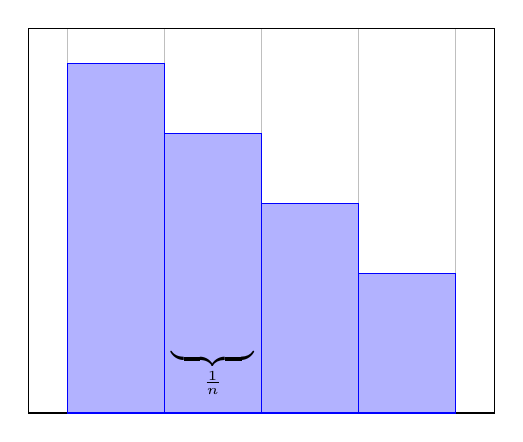
\begin{tikzpicture}
		\begin{axis}[ybar interval, ymax=55,ymin=0, ticks=none, width=7.5cm]
			\addplot coordinates { (10, 50) (15, 40) (20, 30) (25, 20) (30,10) };
			
			\node[label={$ \underbrace{\qquad \quad}_{\frac{1}{n}} $},inner sep=2pt] at (axis cs:17.5,0) {};
		\end{axis}
	\end{tikzpicture}
	
	
	L'area del rettangolo è uguale alla probabilità che assuma un certo valore. 
	Abbiamo visto per Stirling che $ u_{2n} \approx \frac{1}{\sqrt{\pi n}} $. 
	Supponiamo $ n $ grande e $ 0 \le k \le n $; allora possiamo scrivere:
		$$ u_{2k} u_{2n-2k} \approx \frac{1}{2\pi}\frac{1}{\sqrt{k(n-k)}} $$
	
\end{multicols}

Riscriviamo la funzione in termini di $ x $ e chiamiamola $ g $:

$$ g(x) \approx \frac{1}{n2\pi} \frac{1}{\sqrt{x(1-x)}} $$

Da questa formula si vede che l'istogramma è vicino alla funzione $ \frac{1}{2\pi\sqrt{x(1-x)}} $:

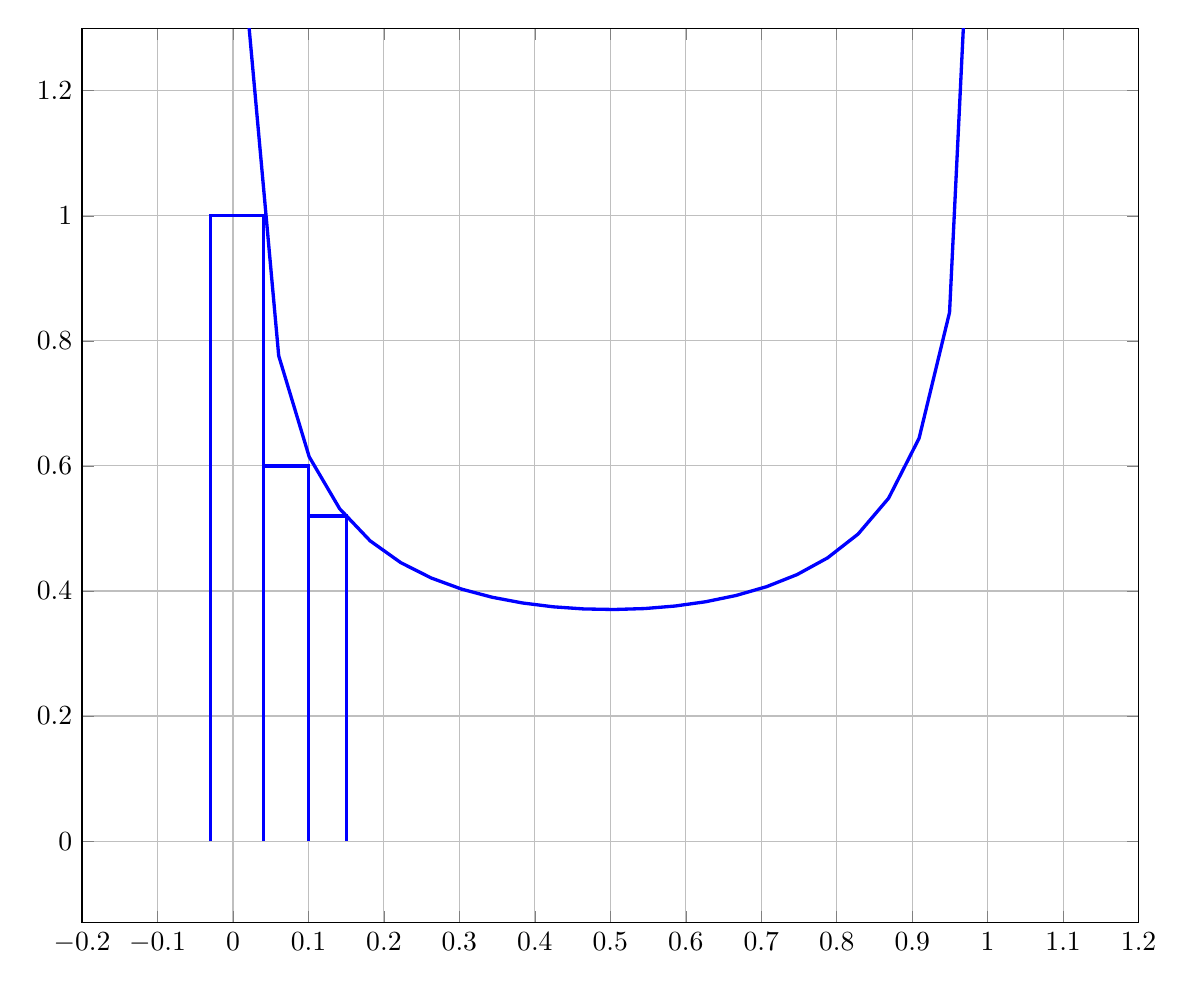
\begin{tikzpicture}
	\begin{axis}[grid=major, width=15cm, xmin=-0.2, xmax=1.2, ymax=1.3]
		%\addplot coordinates { (0, 5) (5, 35) (10, 50) (15, 30) (20, 15) (25, 0) };
		
		\addplot[color=blue, very thick, domain=-2:2, samples=100]	
		{1/(2 * 2.7 *sqrt(x*(1-x)) )};
		
		\addplot [color=blue, very thick] coordinates { (-0.03, 0) (-0.03, 1) (0.04, 1) (0.04, 0) };
		\addplot [color=blue, very thick] coordinates { (0.04,0) (0.04, 0.6) (0.1, 0.6) (0.1, 0)};
		\addplot [color=blue, very thick] coordinates { (0.1, 0) (0.1, 0.52) (0.15, 0.52) (0.15, 0) };

	\end{axis}
\end{tikzpicture}

Dobbiamo fare la somma di tutti i rettangoli sotto la funzione $ \frac{1}{2\pi\sqrt{x(1-x)}} $. Questa è la somma di Riemann, un'approssimazione dell'integrale:
$$ \approx \sum_{\frac{1}{2} < x < z} \frac{1}{n2\pi} \frac{1}{\sqrt{x(1-x)}} $$
$$ \to_{n \to \infty} \int_{\frac{1}{2}}^{z} \frac{1}{\pi \sqrt{x(1-x)}} dx$$ 

Con riferimento al grafico precedente, si vede che quando $ x $ tende a 0 oppure a 1, la probabilità tende all'infinito, mentre a $ \frac{1}{2} $ è nel punto più basso. 

Questa è detta \textbf{prima legge dell'arcoseno} perché la primitiva dell'integrale è uguale a:
$$ \int \frac{1}{\pi \sqrt{x(1-x)}} dx = 2\pi^{-1} \arcsin {\sqrt{x}} + c$$
%TODO controlla sia \pi^{-1}

La prima legge dell'arcoseno è un'approssimazione della probabilità che uno dei due giocatori sia in vantaggio una certa percentuale di volte, per un $ n $ grande. 

Questo vale per la passeggiata aleatoria asimmetrica libera. 
\\
\\
\\
\\
\\
\\
Vediamo un caso simile: consideriamo la probabilità che il primo giocatore sia in vantaggio per un tempo $ 2k $ e che a $ 2n $ la passeggiata sia 0, ovvero i due giocatori siano in pareggio; definiamo

\formule {(   \frac{1}{2^{2n}}) (L_{2k,2n}) = } { probabilità che il primo giocatore  sia in vantaggio per un tempo $ 2k $ e che $ s_{2n} = 0 $}

$ L_{2k, 2n} $ è il numero dei cammini; dividendolo per il numero totale dei cammini $ 2^{2n} $ dà la probabilità. 

Allora $ L_{2k, 2n} = L_{2n} $, e avevamo definito $ L_{2n} = \ddfrac{1}{n+1}	\binom{\displaystyle 2n}{\displaystyle n} $.

È possibile dimostrare che il numero dei cammini non dipende da $ k $, ma è lo stesso per tutti i valori di $ k $; qualsiasi percentuale ha la stessa probabilità.

\paragraph{Dimostrazione} per induzione su $ n $:
\begin{multicols}{2}
	\begin{tikzpicture}
		\begin{axis} [axis equal, axis lines=middle , ticks = none, ymin = 0, ymax = 7, xmin = -3, xmax = 20, width=7.5cm, height=6cm]
			\addplot [color = black] coordinates { (0,0) (2,2) (4,0) (8,4) (9,3) 
							(10,4) (14,0) (16,2) (18, 0)};
			\node [ label=below left:0 ] at (axis cs:0,0) {};
			\node [ label=below: $ 2n $ ] at (axis cs:18,0) {};
		\end{axis}
	\end{tikzpicture}
	
	
	Supponiamo sia vero per $ n-1 $; vogliamo vedere che la proprietà vale anche per $ n $
	%TODO supponiamo sia vero che cosa?
	Supponiamo $ k = n $. Dobbiamo contare i cammini che tornano a 0 e sono sempre $ \ge $ 0; ma lo abbiamo già visto: i cammini sono $ L_{2n, 2n} = \ddfrac{1}{n+1}\binom{\displaystyle n}{\displaystyle n} $.


	Anche il caso $ k = 0 $ lo abbiamo già visto. 
	
\end{multicols}

Supponiamo $ 1 \le k \le n-1 $. Questo cammino deve passare per forza per 0, perché una parte del tempo è in vantaggio il primo giocatore, l'altra il secondo. Sia $ 2r $ il primo istante in cui la passeggiata passa per lo 0. Fino al tempo $ 2r $, il cammino può essere positivo o negativo. 

$$ L_{2k,2n} = \sum_{r=1}^{k} L_{2r-2} L_{2n-2r} + \sum_{r=1}^{n-k} L_{2r-2} L_{2n-2r}$$

%TODO controlla equazione

Modifichiamo la variabile $ r $ al secondo membro, con $ \rho = n -r + 1 $. Quindi 
\begin{align*}
	& \text{per } r = n - k, & \qquad \rho = k + 1 \\
	& \text{per } r = 1, & \qquad \rho = n
\end{align*}

$$ = \sum_{r=1}^{k}L_{2n-2}L_{2n-2r} + \sum_{\rho = k+1}^{n} L_{2\rho - 2} L_{2n - 2\rho}$$

$$ = \sum_{r=1}^{n} L_{2r-2}L{2n-2r} \qed$$

Abbiamo dimostrato che $ L_{2k,2r} $ non dipende da $ k $, ma è uguale per tutti i valori. Ma quanto vale effettivamente?

$ L_{0, 2n} = L_{2n,2n} = L_{2n} $

$ L_{k,2n} $ per $ k = 1, n = 1 $ sono uguali

Supponiamo che: 
$$ \sum_{k=0}^{n} L_{2k,2n} = \binom{2n}{n} $$
facendo variare $ k $ da 0 a $ n $ otteniamo tutti i cammini di lunghezza $ 2n $

Supponiamo $ 1 \le k \le n-1 $:

\begin{align*}
	L_{2k, 2n} & = \frac{\binom{2n}{n} - 2L_{2n}}{n-1} = \\
	& = \frac{\binom{2n}{n} - \frac{2\binom{2n}{n}}{n+1}}{n-1} = \binom{2n}{n} \frac{1 - frac{2}{n+1}}{n-1} \\
	& = \binom{2n}{n}\frac{\frac{n+1-2}{n+1}}{n-1} = \frac{\frac{2n}{n}}{n+1} \\
	& = L_{2n}
\end{align*}

\section{Problema della rovina del giocatore (gambler's ruin)}
Consideriamo un altro problema, la rovina del giocatore. È sempre basato su una passeggiata aleatoria. Consideriamo 2 giocatori A e B che tirano una moneta; se esce testa, A vince 1 euro; se esce croce, perde 1 euro (e lo vince B). Ci chiediamo quale sia il capitale del primo giocatore dopo un certo numero di giocate. 

Supponiamo che al tempo 0 il capitale iniziale di A sia $ x $, mentre il capitale di B ammonti a $ N - x $. Il capitale totale (capitale di A + capitale di B) ammonta quindi a $ N $. Se il capitale di uno dei due giocatori arriva a 0, il gioco si ferma (e si ha la rovina del giocatore). 

Considereremo anche il caso della \textbf{moneta non simmetrica}, dove cioè la probabilità $ p $ che esca testa è $ 0 < p < 1 $. I lanci sono indipendenti tra loro.

Ci chiediamo qual è la probabilità che dopo un certo numero di giocate A oppure B sia rovinato. Non supponiamo ci sia un numero finito di lanci, il gioco potrebbe teoricamente continuare all'infinito. 

Definiamo le seguenti quantità:
\formule{E_i = }{i-esimo lancio è testa (evento)}

$$ P(E^*_1, ..., E^*_n) = p^k(1-p)^{n-k} $$


\begin{equation}
	E^*_i=
	\begin{cases}
		E_i, & \text{se l'evento è verificato}  \\
		\tilde{E}_i, & \text{altrimenti}
	\end{cases}
\end{equation}

Con $ k $ numero degli eventi $ E_i $ e $ n-k $ numero degli eventi $ \tilde{E}_i $.

Questo schema di Bernoulli formalizza il fatto che i lanci siano indipendenti. 

Definiamo

\formule{u_x = }{probabilità di rovina del giocatore A con capitale iniziale $ x $, contro B con capitale iniziale $ N-x $}

\paragraph{Caso simmetrico } $ p = \ddfrac{1}{2} $

Supponiamo $ 0 < x < N $. Osserviamo in generale che $ u_0 = 1 $ e $ u_N = 0 $.

Possiamo scrivere $ u_x $ come la probabilità di rovina del giocatore sapendo che il primo lancio ha dato testa sommata alla probabilità di rovina del giocatore sapendo che il primo lancio ha dato croce:
\begin{align*}
	u_x & = p\cdot u_{x+1} + (1-p)\cdot u_{x-1} \\
	& = \frac{1}{2}u_{x-1} + \frac{1}{2}u_{x+1} = \cancel{\frac{1}{2}}(u_{x+1} - u_{x}) = \cancel{\frac{1}{2}}(u_x - u_{x-1}) \\
	& u_{x+1} - u_x = c \text{ \qquad (la differenza tra due valori successivi è sempre uguale, la chiamiamo } c) \\ \\
	0 & = u_n = u_0 + \sum_{x=0}^{N-1}(u_{x+1} + u_x)\\
	0 & = u_n = 1 + N_c \Rightarrow c = -\frac{1}{N} \\
	u_x & = u_0 + \sum_{y=0}^{x-1} (u_{y+1} - u_y) = 1 - \frac{x}{N}
\end{align*}

Quindi se $ x \to N $, la probabilità che A si rovini tende a 0. Cosa succede se $ N $ tende all'infinito? A parte da $ x $, e B da $ N - x $. La probabilità di rovina in questo caso tende a 1. 

La probabilità che il gioco continui all'infinito è 0.

\paragraph{Caso non simmetrico} $ 0 < p < 1 $
Nel caso $ p = \ddfrac{1}{2} $ le differenze erano uguali (al valore $ c $). Nel caso non simmetrico questo non vale. Occorre introdurre la \textbf{somma geometrica}:

supponiamo $ \alpha \ne 1 $:
\begin{align*}
	S & = \sum_{k=0}^n \alpha^k = \ddfrac{\alpha^{n+1} - 1}{\alpha - 1} \\
	\alpha S & = S - 1 + \alpha^{N+1} - 1 \\
	(\alpha - 1)S & = \alpha^{N+1} - 1 \\
	S & = \ddfrac{\alpha^{N+1} - 1}{\alpha - 1} \qquad \qquad \begin{cases}
		\alpha < 1, & \text{la serie è convergente} \\
		\alpha > 1, & \text{la serie va avanti all'infinito}
	\end{cases}
\end{align*}

Tornando a noi, abbiamo detto che nel caso simmetrico $ 0 < p < 1 $; se $ p > \ddfrac{1}{2} $ A è favorito, altrimenti è favorito B. Sia ancora $ u_x $ la probabilità di rovina di A, e scriviamola ancora come la somma delle probabilità della rovina del giocatore se il primo lancio è testa oppure è croce:
$$ 0 < x < N \qquad \qquad \qquad u_x = p\cdot u_{x+1} + q\cdot u_{x-1} $$
Con $ q = 1-p $. 

\begin{align*}
	(p+q)u_x & = pu_x + q_ux = pu_{x+1} + qu_{x-1} \\
	q(u_x - u_{x-1})  & = p(u_{x+1} - u_x) \\
	u_{x+1} - u_x & = \frac{q}{p}(u_x - u_{x-1}) \\
	u_{k+1} - u_k & = (\frac{q}{p})^k(u_1 - u_0) \qquad \qquad u_0 = 1 \text{ (rovina all'istante iniziale), } u_N = 0 \\
	u_k & = u_0 + \sum_{j=0}^{k-1}(u_{j+1} - u_j) \\
	& = 1 + \sum_{j=0}^{k-1}(\frac{q}{p})^j(u_1 - u_0) \\
	& = 1 + (u_1 - u_0) \sum_{j=0}^{k-1} (\frac{q}{p})^j \\
	\text{possiamo} & \text{ applicare la formula della somma geometrica } (p\ne \frac{1}{2} \Rightarrow \frac{q}{p} \ne 1): \\	 
	 & = 1 + (u_1 - u_0)\ddfrac{\left(\ddfrac{q}{p}\right)^k - 1}{\ddfrac{q}{p} - 1}
\end{align*}

Applichiamo la formula per $ k = N $, sapendo che $ u_N = 0 $:

$$ 0 = 1 + (u_1 - u_0) \ddfrac{\left(\ddfrac{q}{p}\right)^N - 1}{\ddfrac{q}{p} - 1} $$

$$ u_1 - u_0 = - \ddfrac{\ddfrac{q}{p} - 1}{\left(\ddfrac{q}{p}\right)^N - 1} $$

Possiamo calcolare $ u_k $ in generale:
$$ u_k = 1 - \ddfrac{\left(\ddfrac{q}{p}\right)^k - 1}{\left(\ddfrac{q}{p}\right)^N - 1} $$

che è la probabilità di rovina di A che parte con capitale iniziale pari a $ k $. 

Consideriamo ora $ v_k $ la probabilità di rovina di B; in questo caso B vince con probabilità $ q $.

$$ v_k = 1 - \ddfrac{\left(\ddfrac{p}{q}\right)^{N-k} - 1}{\left(\ddfrac{p}{q}\right)^N - 1} $$

$ v_k + u_k = 1 $. La probabilità che il gioco continui all'infinito è 0 (uno dei due giocatori va in rovina prima o poi). Cosa succede se $ N \to \infty $ (con $ p \ne \frac{1}{2} $)? Supponiamo $ p > \frac{1}{2} $. 

$$ \frac{q}{p} < 1 \qquad \qquad u_k \stackrel{N \to \infty}{\longrightarrow} \left(\frac{q}{p}\right)^k \qquad (\text{perché} \left(\frac{q}{p}\right)^N \to 0, \text{ perché } \frac{q}{p} < 1) $$

Quindi se A è favorito, la sua probabilità di rovina è minore di 1, e più è grande $ k $ e più si abbassa.

Se $ p < \ddfrac{1}{2} $: $ \ddfrac{q}{p} > 1 $ e $ u_k \stackrel{N \to \infty}{\longrightarrow} 1 $.

\section{Processi di diramazione di Galton-Watson (branching processes)}
Sono esempi particolari delle catene di Markov, un modello più generale. Servono per studiare l'evoluzione di una popolazione. È un modello molto semplificato; partiamo supponendo di avere un solo individuo che avrà un certo numero di figli. 

Supponiamo che ogni individuo abbia le stesse probabilità di avere figli, indipendentemente dagli altri individui, e gli intervalli (numero di figli) siano regolari. Consideriamo una successione di variabili aleatorie, e vogliamo vedere quanti figli ci sono nelle varie generazioni.

Definiamo:
\formule{x_i = }{numero di figli della generazione i-esima}
\formule{p_k = }{probabilità di avere $ k $ figli per ogni individuo; $ \sum_{k=0}^\infty p_k = 1 $ (sono eventi incompatibili, è una partizione).}

Supponiamo che l'attesa del numero di figli sia finita; la indichiamo con $ \mu $:
$$ \mu = \sum_{k=0}^{\infty} k \cdot p_k < +\infty $$

Quindi abbiamo supposto $ x_0 = 1 $. Qual è l'attesa della k-esima generazione?

\begin{tcolorbox}
	\paragraph{Formula delle probabilità totali} date due variabili aleatorie $ A $ e $ B $ , possiamo chiederci quanto vale l'\textit{attesa condizionata}, ovvero la probabilità che si verifichi $ A $ sapendo che $ B $ assume un certo valore $ x $:
		$$ P(A | B = x) $$
	Possiamo conoscere l'attesa non condizionata con la formula delle probabilità totali:
		$$ P(X) = \sum_{x=0}^{\infty} P(A|B=x)P(B=x) $$
\end{tcolorbox}

Siano $ x $ e $ y $ due variabili aleatorie a valori interi. Ci possiamo chiedere l'attesa di $ x $ quando $ y $ assume certi valori: $ P(x | y = j) $; usando la formula delle probabilità totali: 
$$ P(x) = \sum_{j=0}^{\infty} P(x | y = j)P(y=j) $$

Vogliamo calcolare l'attesa di $ k $:
\begin{align*}
	P(x_k) & = \sum_{j=0}^{\infty} P(x_k | x_1 = j)P(x_1 = j) \\
	& = \sum_{j=0}^{\infty} jp_jP(x_{k-1}) \\
	& = \mu P(x_{k-1})
\end{align*}

Possiamo dividere la j-esima generazione nei figli dell'individuo 0; %TODO ah si? ha senso?
possiamo suddividerla in $ j $ sottoinsiemi e calcolare l'attesa dei sottoinsiemi:
$$ P(x_k) = \mu P(x_{k-1}); \qquad \qquad P(x_0) = 1 \text{ (per ipotesi)}; \qquad \qquad P(x_k)=\mu^k$$

Se $\mu < 1$, avremo l'estinzione:
\formule{E_k(x_k=0)}{evento che al tempo $ k $, $ x_k=0 $}
\formule{E_k \subset E_{k+1}}{$ A $ è contenuto in $ B $ se quando si verifica il primo, allora si verifica anche il secondo}
\formule{E = \bigvee_{k=1}^\infty E_k}{si verifica almeno uno degli eventi}

(Nota: $\bigvee$ indica la somma logica, si può usare anche $\bigcup$).
\\
\\
\\
%TODO sugli appunti c'è un titolo: LIQUIDITÀ (?) NUMERABILE
Se abbiamo una successione di eventi crescenti ($ E_k \subset E_{k+1} $), allora
$$ P(E) = \underset{k}{sup} \: P(E_k)$$
Vogliamo mostrare che se $\mu < 1$, allora $ P(E) = 1 $:
\begin{align*}
	P(E_k) & = 1 - P(\tilde{E}_k) \\
	& = 1 - \sum_{j=1}^{\infty}P(x_k = j) \ge 1 - \sum_{j=1}^{\infty}jP(x_k=j) \\
	& = 1 - P(x_k) \\
	& = 1-\mu^k \to 1 \qquad \qquad \text{perché abbiamo supposto } \mu < 1 \Rightarrow \mu^k \stackrel{k \to \infty}{\longrightarrow} 0 \\ \\
	& P(E) = 1
\end{align*}(

Se invece $\mu = 1$, l'attesa di $ x_k(P(x_k)) $ rimane 1.

Vediamo infine il caso generale: non facciamo ipotesi su $\mu$, ma può assumere qualsiasi valore.

Sia $ \Pi^k = P(x_k = 0) $.

Possiamo usare la formula delle probabilità condizionate:
$$ \Pi^k = P(x_k = 0) = \sum_{j=0}^{\infty} P(x_k = 0 | x_1 = j) P(x_1 = j) $$
$$ = \sum_{j=0}^{\infty} p_j\Pi^{(k-1)j} $$  %TODO forse questo p_j è in realtà P_j

%TODO controlla anche che i \Pi non siano in realtà \pi e viceversa (nelle equazioni più in basso)
Affinché nella k-esima generazione non ci siano più individui, in tutti i rami ci deve essere l'estinzione. 

Definiamo una funzione $ f $:
\begin{align*}
	f(s) & = \sum_{j=0}^{\infty} p_j s^j \\
	\pi^k & = f(\pi^{k-1}) \\
	\pi^k \ge \pi^{k-1} \qquad \qquad \pi^k \le 1
\end{align*}

Abbiamo una successione non decrescente:
$$ \pi = P(E) = \underset{k}{sup} \: \pi^k $$

Ipotizziamo che $ p_0 + p_1 < 1 $ e $ p_0 > 0 $.

Se $ p_0 = 0$, vorrebbe dire che la p che un individuo non abbia figli sia 0. Allora ls $ P(E) $ (probabilità di estinzione) sarebbe 0. 

Supponiamo ora $ p_0 + p_1 = 1 $ e $ p_0 > 0 $, ovvero ogni individuo non ha figli, oppure ha un solo figlio: allora $ P(E) = 1 $ (si ha estinzione).

Studiamo com'è fatta $ f(s) $:

$$
\begin{array}{ccc}
	f(1) = 1 & \qquad f'(s) = \sum_{j=1}^{\infty} j \cdot p^j \cdot s^{j-1} & f''(s) > 0 \\
	f(0) = p_0 > 0 & \quad f'(1) = \sum_{j=1}^{\infty} j \cdot p^j = \mu & \quad f''(s) = \sum_{j=2}^{\infty} p_j \cdot j \cdot (j-1) s^{j-2} > 0, \quad 0 < s < 1
\end{array}
$$

La derivata seconda è positiva, quindi la funzione è strettamente convessa.

\begin{tikzpicture}
	\begin{axis}[grid=major, axis lines = middle, width=15cm, xmin=-0.2, xmax=1.2, ymax=1.1, ymin=-0.1, xtick={1}, ytick={1}]
	%xtick={0.417, 0.805, 1}, ytick={0.417, 0.65, 1}
	
		\addplot[color=blue, very thick, domain=0:1, samples=300]	
		{0.4 + 0.6*x*x*x*x}; %Se stai leggendo i sorgenti, questa è una funzione a caso che mi sono inventato
		
		\addplot [color=blue] coordinates { (0, 0.4) (1, 1)};
		\addplot [color=blue, dashed] coordinates { (0,0) (1,1)};
		
		\addplot [color=orange] coordinates { (0.417, 0) (0.417, 0.417) (0.417, 0.65) 
		(0.805, 0.65) };
	
		\addplot [color=orange] coordinates { (0, 0.417) (0.417, 0.417) };
		
		\node [ circle, fill, draw=black, scale=0.5, label=below left:$ p_0 $ ] at (axis cs:0,0.4) {};
		\node [ circle, fill, draw=black, scale=0.5, label=above right:$f(1)$ ] at (axis cs:1,1) {};
		\node [ label=below:$ \pi^{(1)} $] at (axis cs:0.417, 0) {};
		\node [ label=above:$ \pi^* $] at (axis cs:0.805, 0.65) {};
		
	
	\end{axis}
\end{tikzpicture}

Qual è la probabilità di estinzione? $ \pi = f(\pi) $; la probabilità di estinzione è una soluzione di una delle funzioni sottostanti:

$ \pi^{(1)} = p_0 $ (prima generazione)

$ \pi^{(2)} = f(\pi^{(1)}) $

$ \pi^{(3)} = f(\pi^{(2)}) $

$ \pi^{(k+1)} = f(\pi^{(k)}) $

Siccome $ f $ è crescente, se applichiamo da entrambe le parti:

$ p_0 < \pi^* $

$ \pi^{(1)} < \pi^* $

...

$ \pi^t < \pi^* $

Questa successione rimane sempre più piccola di $\pi^*$, quindi il limite tenderà a $ \pi^* $, che è minore di 1.

Quindi se $ \mu > 1$, c'è una probabilità positiva che non ci sia estinzione. 
%TODO qualcosa non torna: \mu è la probabilità di estinzione, secondo me la frase sopra è "se ??? > 1, allora \mu < 1 (cioè c'è una probabilità positiva che non si estinugano - ovvero 1 - \mu)

%TODO manca grafico con caso \mu >= 1

\paragraph{Esempi} vediamo alcuni esempi:
\begin{itemize}
	\item $ p_0 = \frac{1}{2}, p_1 = \frac{1}{4}, p_2 = 0, p_3 = \frac{1}{4} $
	
	$ \mu = 0 \cdot \frac{1}{2} + 1 \cdot \frac{1}{4} + 2 \cdot 0  + 3 \cdot \frac{1}{4} = 1 \Rightarrow \pi = 1$
	\item $ p_0 = \frac{1}{3}, p_1 = \frac{1}{3}, p_2 = 0, p_3 = \frac{1}{3} $
	
	$ \mu = 0 \cdot \frac{1}{3} + 1 \cdot \frac{1}{3} + 2 \cdot 0  + 3 \cdot \frac{1}{3} = \frac{4}{3} > 1$
	
	Per calcolare $\pi$ dobbiamo risolvere:
	\begin{align*}
		f(s) - s & = 0 \Rightarrow f(s) = \frac{1}{3} + \frac{s}{3} + \frac{s^3}{3} \\
		& \frac{s^3}{3} + \frac{s}{3} + \frac{1}{3} - s = 0 \\
		& \frac{s^3}{3} - \frac{2}{3}s + \frac{1}{3} = 0 \\
		& s^3 - 2s + 1 = 0 \Rightarrow (s-1)(s^2 - As + C) = 0
	\end{align*}
	
	Quindi $ s = 1 $ è una soluzione; risolvendo il secondo elemento dell'equazione otterremo 2 radici, una di queste comprese tra 0 e 1, che è quella che ci interessa. 
	
	\item $ p_0 = \frac{1}{4}, p_1 = \frac{1}{4}, p_2 = \frac{1}{4}, p_3 = \frac{1}{4} $
	
	\begin{align*}
		f(s) & = \frac{1}{4}(s^3 + s^2 + s + 1) \\
		& \frac{1}{4}s^3 + \frac{1}{4}s^2 + \frac{1}{4}s + \frac{1}{4} = 0 \\
		& s^3 + s^2 - 3s + 1 = 0 \\
		& (s-1)(s^2 + As + B) = 0	
	\end{align*}
	
	Soluzione come nel caso precedente. 
\end{itemize}

\section{Simulatori}
Supponiamo di voler generare una passeggiata aleatoria simmetrica tra 0 e $ 2n $. Prendiamo una successione $ x_1, ..., x_{2n} $. Definiamo una nuova variabile $ z_i $:

$$
z_i =
\begin{cases}
	1, & \text{per } x_i > \frac{1}{2}\\
	-1, & \text{per } x_i \le \frac{1}{2}
\end{cases}
$$

Definiamo $ S_k = z_1 + ... + z_k $.

Facciamo tante prove e vediamo quante passeggiate sono positive: la percentuale del numero di passeggiate aleatorie sempre positive dovrebbe tendere valore delle probabilità che una passeggiata sia sempre positiva per la legge dei grandi numeri. 

Si può mostrare un altro esempio per la rovina del giocatore: questo problema si può vedere una passeggiata aleatoria in generale non simmetrica. In questo caso, a differenza di prima, teoricamente potremmo continuare all'infinito. Prendiamo la successione $ x_1, x_2, ... $ e definiamo:

$$
	z_i =
	\begin{cases}
		1, & \text{per } 0 < x_i \le p\\
		-1, & \text{per } p < x_i < 1
	\end{cases}
	\qquad \qquad s_n = x + z_1 + ... + z_n
$$

Con $ 0 < x < n $. Quindi la passeggiata parte da un certo $ 0 < x < N $ e ogni volta che genero $ z_n $ vado avanti. Se $ z_n = 0 $ ho la rovina del giocatore A, se $ z_n  = N $ ho la rovina di B, altrimenti genero un altro numero. Sappiamo che con $ p = 1 $ prima o poi ci fermeremo. 

Se facciamo il rapporto tra il numero di volte che A si è rovinato e le passeggiate totali, facendo infinite prove, il valore dovrebbe tendere alla probabilità di rovina di A. 

Si può vedere anche per i processi di diramazione. Supponiamo di essere nell'intervallo $ [0,1] $ e di dividerlo in tanti intervalli più piccoli, supponendo che un individuo possa avere $ k $ figli: $ p_0, p_1, ..., p_k  \in [0,1]$. I $ k+1 $ intervalli hanno lunghezza pari alla loro probabilità. 

Scegliamo, per il primo individuo, un intervallo a caso; diciamo che esca $ p_i $: il primo individuo avrà i figli. Ripetiamo per ogni individuo della seconda generazione, e così via. Tipicamente la probabilità di estinzione è minore di 1; l'estinzione avviene nelle prime generazioni (perché la prole cresce esponenzialmente ed è più difficile che avvenga).

Questi tre esempi appena illustrati sono un caso particolare di un modello più generale detto \textbf{catene di Markov}. 

\chapter{Catene di Markov}
\section{Catene di Markov omogenee}
Se ripensiamo ai problemi e ai modelli visti precedentemente, la caratteristica comune è che se sappiamo la posizione in un certo istante, possiamo calcolare la probabilità di andare nello stato successivo, poiché questa probabilità è appunto indipendente dalle misurazioni precedenti. Questa proprietà è chiamata \textbf{proprietà di Markov}.

Studieremo le \textbf{catene di Markov omogenee con numero finito o numerabile di stati}.

L'attributo "omogeneo" indica che la probabilità di passare da uno stato all'altro. Esistono anche fenomeni dipendenti dal tempo (es. se studiamo la temperatura, bisogna tenere conto di in quale giorno dell'anno si stanno effettuando le misurazioni, e non è quindi un fenomeno omogeneo nel tempo).

Lo "stato", nel caso della probabilità aleatoria, è il punto in cui ci troviamo. Possiamo rappresentare lo stato con un numero intero, che quindi può assumere infiniti valori numerabili. Nel caso dei processi di diramazione, ad esempio, lo stato può essere il numero degli individui (un intero non negativo). 

Per \textbf{definire} una catena di Markov occorre quindi indicare:
\begin{enumerate}
	\item $S$: spazio degli stati, finito o numerabile;
	\item \textbf{distribuzione iniziale} $ u_s $: valori compresi tra 0 e 1 tali che la loro somma è 1. La distribuzione iniziale ci dice al tempo 0, supponendo che il tempo sia discreto, qual è la probabilità di trovarci in un certo stato. Possiamo prendere come stato iniziale qualsiasi stato oltre a 0;
	$$ 0 \le u_s \le 1 \qquad \qquad \sum u_s  = 1 \qquad \qquad s \in S $$
	\item \textbf{probabilità di transizione}: è una matrice; siccome $ S $ può essere infinito, anche questa matrice può avere infinite righe e colonne. Indica la probabilità di passare da uno stato $ s $ di partenza ad uno stato $ s' $ d'arrivo:
	$$ s, s' \in S \qquad \qquad \forall s \sum_{s'\in S} p_{s,s'} = 1 $$
\end{enumerate}

Possiamo definire una successione $ x_0, x_1, x_2, ... $ e, dopo aver definito anche i 3 parametri sopra descritti, possiamo dare una distribuzione delle variabili aleatorie. Dato $ n $ finito, e $ p $, possiamo definire la distribuzione di $ x_0, x_1, ... $:

\begin{align*}
	& P(x_0 = s_0, x_1 = s_1, ..., x_n = s_n) \\
	= & u_{s_0} \cdot p_{s_0, s_1} \cdot u_{s_1} \cdot p_{s_1, s_2} \cdot ... \cdot p_{s_{n-1}, s_n}
\end{align*}

C'è un problema di compatibilità: se assegno la distribuzione dei primi $ n+1 $, posso sapere la distribuzione dei primi $ n $. %TODO che cacchio vuol dire

\textbf{Distribuzione marginale} (dei primi $ n $): si calcola facendo la somma dei primi $ n+1 $ valori. 

Devo verificare quindi che l'equazione sopra sia valida. %TODO ????
Queste assegnazioni delle probabilità sono compatibili, è coerente. 

\subsection{Proprietà di Markov}
Supponiamo di avere una successione $ s_0, ..., s_{n-1}, s $
e che $ u_{s_0} \cdot p_{s_0, s_1} \cdot p_{s_1, s_2} \cdot ... \cdot p_{s_{n-1}, s}  > 0 $ (se il prodotto fosse 0, la probabilità che si verifichi la successione sarebbe 0). 
Ci chiediamo quanto vale la seguente probabilità:
$$ P(x_{n-1} | x_0 = s_0, x_1 = s_1, ..., x_{n-1} = s_{n-1}, x_n = s) $$

Usiamo la formula della probabilità condizionata (richiamo: dati due eventi $ A, B $: $ P(A|B) = \frac{P(AB)}{P(B)} $, con $ P(B) > 0 $):

\begin{align*}
	& = \frac{P(x_0 = s_0, ..., x_{n-1} = s_{n-1}, x_n = s, x_{n-1} = s')}{P(x_0 = s_0, ..., x_{n-1} = s_{n-1}, x_n = s)} \\
	& = \frac{u_{s_0}\cdot p_{s_0, s_1} \cdot ... \cdot p_{s_{n-1}, s} \cdot p_{s,s'}}{u_{s_0}\cdot p_{s_0, s_1} \cdot ... \cdot p_{s_{n-1}, s} \cdot p_{s_{n-1},s}}\\
	& = p_{s,s'}
\end{align*}

Quindi, se voglio calcolare la probabilità di andare da $ s $ a $ s' $ mi basta conoscere l'ultimo stato, sapere tutto quello che è successo prima è irrilevante. 

Qual è la probabilità di transizione in più passi, ad esempio in due passi?

\begin{align*}
	& P(s_2 = s' | x_0 = s) \\
	& = \frac{P(x_0 = s, x_2 = s')}{P(\underbrace{x_0 = s}_{\substack{ = u_s \\ \text{distribuzione} \\ \text{iniziale}}}  )} \\
	& = \frac{\sum_{s'' \in S} P(x_0 = s, x_1 = s'', x_2 = s')}{P(x_0 = s)} \\
	& = \frac{\sum_{s'' \in S} u_s p_{s, s''} p_{s'', s'}}{u_s} \\
	& = \sum_{s'' \in S} p_{s,s''}p_{s'', s'} \\
	& = p_{s, s''}^{(2)} \qquad \qquad \qquad \text{(probabilità di transizione in 2 passi)}
\end{align*}

Supponendo di partire in un tempo arbitrario $\ne 0$, la notazione diventa:
 $$ p_{s,s'}^{(2)} = P(x_{k+2} = s' | x_k = s)$$

Se immaginiamo di rappresentare $ p_{s,s'} $ come una matrice, $ p^{(2)} $ è il prodotto riga colonna della matrice per se stessa:
$$ p_{s,s'}^{(2)} = (\Pi^2)_{s,s'}$$

Generalizzando:
$$ P(x_{k+n} = s' | x_k = s) = (\Pi^n)_{s,s'} $$

Quindi mi basta moltiplicare la matrice $ n $ volte e il risultato corrisponderà all'elemento corrispondente alla riga $ s $ e alla colonna $ s' $. 

\paragraph{Esempio 1} Vediamo un esempio di matrice. Supponiamo di avere due stati; la matrice avrà dimensione $ 2 \times 2 $; la somma degli elementi sulla matrice deve dare 1:

$$ 
	\begin{array}{c}
		S = {0, 1} \\
		0 < p < 1
	\end{array}
	\qquad \qquad \qquad \Pi = \left(\begin{array}{cc}
	 	p & 1-p \\
	 	q & 1-q
	\end{array}\right)
$$

$ p $ è la probabilità di passare dallo stato 0 allo stato 0; $ 1-p $ è la probabilità di passare dallo stato 0 allo stato 1.

Possiamo finalmente calcolare le probabilità di passare da uno stato all'altro in $ n $ passi:

\begin{align*}
	p_{0,0}^{(n)} \qquad \qquad \qquad \Pi^{n+1} = \; & \Pi^n \Pi \\
	p_{0,0}^{(n+1)} = \; & p_{0,0}^{(n)}p + p_{0,1}^{(1-p)} \\
	= \; & p_{0,0}^{(n)}p + (1-p_{0,0}^{(n)})(1-p)  \\ \\
%	\text{Sono tutti eventi incompatibili, la } & \text{loro somma deve fare 1} \\ \\
	p_{0,0}^{(n+1)} = \; & p_{0,0}^{(n)}(p-1-q) + (1-q)  \\
	p_{0,0}^{(2)} = \; & p(p+q-1) + (1-q) 
\end{align*}

Il calcolo è lasciato per esercizio (è una somma geometrica nota, $ p_{0,1}^{(n)} = 1-p^{n} $)

\paragraph{Esempio 2} Consideriamo una passeggiata aleatoria nel caso generale (non simmetrico). Sia $ 0 < p < 1 $ la probabilità di fare un passo a destra. 

$$ 
	\begin{array}{cc}
	S = Z & u_0 = 1, u_s = z \\
	 & \text{per } s \ne 0 \\
	 & \\
	p_{s,s_0} = p & p_{s,s-1} = 1-p \\
	p_{s,s'} = 0 & s' + s+1 = s-1
	\end{array}
$$

Esempio: 

$ p_{s,s}^{(2)} = p(1-p) + (1-p)p = 2p(1-p) $

Ci sono solo 2 possibilità: faccio prima un passo a sinistra e poi a destra, oppure il contrario. 

$ p_{s, s+2}^{(2)} = p^2 \cdot p_{s,s-2}^{(2)}  = (1-p)^2$ 

$ p_{s,s'}^{(2)} = 0 \qquad \qquad \text{per } s \ne s', s+2, s-2$

Anziché considerare la passeggiata aleatoria su $\mathbb{Z}$, posso considerare un intervallo finito $ [a,b] \subset \mathbb{Z} $; devo però definire cosa succede agli estremi dell'intervallo. 

\textbf{Condizioni periodiche}: danno un senso orario o antiorario. Se sono in $ a $ e faccio un passo a sinistra, vado in $ b $:

$$  \substack {\displaystyle a < s < b \; , \qquad \qquad p_{s,s+1} = p \; , \qquad  \qquad p_{s,s-1} = 1-p \\ \\ \\
	\begin{array}{cccccc}
		p_{a,b} = 1-p & & & & & p_{a, a+1} = p \\
		p_{b,a} = p & & & & & p_{b, b-1} = 1-p
	\end{array} }
 $$ 

\subsection{Modello di Ebembat} %TODO ??? cerca nome di sto modello

Descrive la componente di un gas. Supponiamo di avere $ n $ particelle; gli stati saranno $ S = \{0, 1, ... N \} $.

\begin{multicols}{2}
	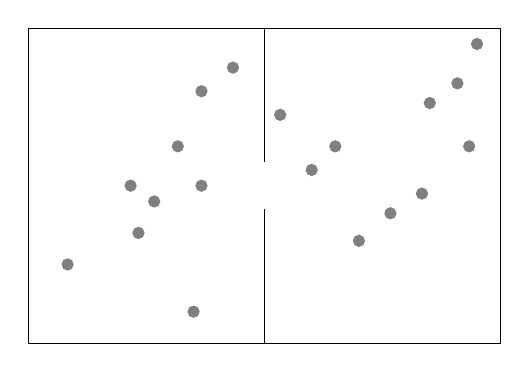
\begin{tikzpicture}
		\draw (0,0) -- (6,0) -- (6,4) -- (0,4) -- (0,0);
		\draw (3,0) -- (3,1.7);
		\draw (3,2.3) -- (3,4);
		
		\filldraw [gray] (0.5,1) circle (2pt);
		\filldraw [gray] (2.2,2) circle (2pt);		
		\filldraw [gray] (1.4,1.4) circle (2pt);
		\filldraw [gray] (2.6,3.5) circle (2pt);
		\filldraw [gray] (1.9,2.5) circle (2pt);
		\filldraw [gray] (2.1,0.4) circle (2pt);
		\filldraw [gray] (1.3,2) circle (2pt);
		\filldraw [gray] (2.2,3.2) circle (2pt);
		\filldraw [gray] (1.6,1.8) circle (2pt);
		%\filldraw [gray] (0.6,2.8) circle (2pt);
		
		\filldraw [gray] (4.2,1.3) circle (2pt);
		\filldraw [gray] (5.6,2.5) circle (2pt);
		\filldraw [gray] (4.6,1.65) circle (2pt);
		\filldraw [gray] (5.1,3.05) circle (2pt);
		\filldraw [gray] (3.2,2.9) circle (2pt);
		\filldraw [gray] (5,1.9) circle (2pt);
		\filldraw [gray] (3.6,2.2) circle (2pt);
		\filldraw [gray] (5.45,3.3) circle (2pt);
		\filldraw [gray] (3.9,2.5) circle (2pt);
		\filldraw [gray] (5.7,3.8) circle (2pt);
		
	\end{tikzpicture}
		
	Le probabilità che una particella vada a destra o a sinistra sono rispettivamente:
	$$ p_{s,s+1} = \frac{N-s}{N} $$
	$$ p_{s,s-1} ??? $$ %TODO
	
\end{multicols}

\subsection{Modello di Bernoulli-Laplace}

Descrive l'evoluzione di un gas; in questo caso abbiamo 2 gas diversi, A e B, ed $ N $ particelle del gas A e altrettante del gas B.

\begin{center}
	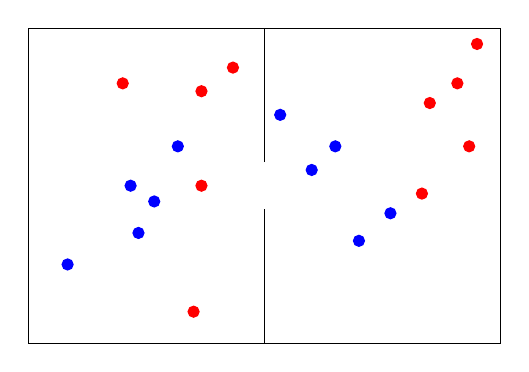
\begin{tikzpicture}
		\draw (0,0) -- (6,0) -- (6,4) -- (0,4) -- (0,0);
		\draw (3,0) -- (3,1.7);
		\draw (3,2.3) -- (3,4);
		
		\filldraw [blue] (0.5,1) circle (2pt);
		\filldraw [red] (2.2,2) circle (2pt);		
		\filldraw [blue] (1.4,1.4) circle (2pt);
		\filldraw [red] (2.6,3.5) circle (2pt);
		\filldraw [blue] (1.9,2.5) circle (2pt);
		\filldraw [red] (2.1,0.4) circle (2pt);
		\filldraw [blue] (1.3,2) circle (2pt);
		\filldraw [red] (2.2,3.2) circle (2pt);
		\filldraw [blue] (1.6,1.8) circle (2pt);
		\filldraw [red] (1.2,3.3) circle (2pt);
		
		\filldraw [blue] (4.2,1.3) circle (2pt);
		\filldraw [red] (5.6,2.5) circle (2pt);
		\filldraw [blue] (4.6,1.65) circle (2pt);
		\filldraw [red] (5.1,3.05) circle (2pt);
		\filldraw [blue] (3.2,2.9) circle (2pt);
		\filldraw [red] (5,1.9) circle (2pt);
		\filldraw [blue] (3.6,2.2) circle (2pt);
		\filldraw [red] (5.45,3.3) circle (2pt);
		\filldraw [blue] (3.9,2.5) circle (2pt);
		\filldraw [red](5.7,3.8) circle (2pt);
	
	\end{tikzpicture}
\end{center}

Supponiamo che in ogni istante sia scelta a caso una particella nel contenitore sinistro, una a caso nel contenitore destro e vengano scambiate. 

Lo stato $ S = \{0, 1, ..., N\} $ rappresenta il numero di palline di gas A a sinistra. 

$ p_{s,s} $ è la probabilità che ci siano $ n $ particelle A a sinistra e che dopo lo scambio questo valore rimanga invariato; questo può capitare se scambiamo una particella di A a sinistra con un'altra particella, sempre di A, a destra (oppure se scegliamo due particelle di tipo B).

$ p_{s,s} = ??? $ %TODO

$ p_{s,s-1} = \frac{s}{N}\cdot \frac{s}{N} = \frac{s^2}{N^2} ???$ %TODO

\section{Classificazione degli stati}

Due stati $ s $ e $ s' $ si dicono \textbf{comunicanti} quando $ s $ comunica con $ s' $, ovvero la probabilità di andare da $ s $ a $ s' $ è positiva:

$ p^{n}_{s,s'} = 0 $

$ p^{(???)}_{s,s'} = 0 $, con $ s' \ne s $ %TODO

Uno stato comunica con sè stesso. 

\paragraph{Definizione} (più precisa) Uno stato $ s $ comunica con uno stato $ s' $ se esiste $ n $ tale che la successione da $ s $ a $ s' $ in $ n $ passi è sempre positiva ??? %TODO

\paragraph{Proprietà} Siano $ s $ e $ s' $ due stati comunicanti: $ s \prec s' $

Se $ us < s' $ e $ s' < s'' $ %TODO controlla abbia senso (riguarda lezione)
, allora $ s \prec s'' $ \\
\\
In generale, se ho due cammini:

$ s, s_1, ..., s_{n-1}, s'' $

$ s', \bar{s}_1, ..., \bar{s}_{m-1}, s'' $
\\
Allora possiamo metterli insieme e fare un cammino che colleghi $ s, s''$. \\
\\
\\
Partendo dalla nozione di comunicazione possiamo definire una \textbf{relazione di equivalenza}. Nota: la comunicazione non è simmetrica. 

$ s \simeq s' $ se $ s \prec s' $ e $ s' \prec s $
\\
$ s \prec s $ perché lo stato comunica sempre con sè stesso.

Proprietà transitiva: se $ s \simeq s' $ e $ s' \simeq s'' $, allora $ s' \simeq s'' $

Proprietà simmetrica: $ s \simeq s' $ e $ s' \simeq s $
\\
\\
Abbiamo una relazione di equivalenza, possiamo definire una classe di equivalenza:
$$ [s] = \{s' | s' \simeq s\} $$

La nozione di comunicazione si può estendere alle classi di equivalenza:
$$ [s] \prec [s'] \text{ se } s \prec s'$$

Una classe equivalente ad $ s $ si dice \textbf{massimale} se non comunica con un'altra classe di equivalenza. 

Quando la catena di Markov arriva in uno stato che appartiene ad una classe massimale, rimane "bloccata" sempre dentro stati di quella classe. 

Una catena di Markov si dice \textbf{irriducibile} se da una sola classe di equivalenza ??? %TODO

cioè lo spazio degli eventi $ S $ è una sola classe di equivalenza.
\\
\\
Consideriamo la passeggiata aleatoria su $ [a,b] \subset \mathbb{Z} $ con condizioni assorbenti:

$$ a < s < b \qquad \qquad \begin{array}{c}
 	p_{s,s+1} = p \\
    p_{s,s-1} = 1-p
\end{array}$$

$$ \begin{array}{cc}
	p_{a,a} = 1 & p_{a,s} = 0 \\
	p_{b,b} = 1 & p_{b,s} = 0
\end{array}$$

Ovvero, se partiamo da uno stato interno lo spostamento è "normale", mentre se siamo in $ a $ o $ b $ rimaniamo sempre in quello stato (come ad esempio nella rovina dei giocatori). 

\paragraph{Esempio} Definiamo ora 3 classi di equivalenza:
$$ c_1 = \{a\} \quad c_2 = \{a+1, ..., b-1\} \quad c_3 = \{b\}, \qquad c_2 \prec c_1, c_2 \prec c_3$$ 

$ c_1 $ e $ c_3 $ sono massimali. In questo caso la catena di Markov non è irriducibile (il modello di Bernoulli-Laplace è un esempio di catena irriducibile). 

\paragraph{Periodo} Dato uno stato $ s \in S $:

$$ A^+_s = \{? | p_{s,s}^{(n)} > 0\} $$ %TODO
$$ A^+_s \ne 0 $$

Se $ n_1 \in A^+_s $ e $ n_2 \in A^+_s $, allora $ n_1 + n_2 \in A^+_s $

(ovvero la probabilità di andare dallo stato $ s $ allo stato $ s $ in $ n_1 + n_2 $ passi è positiva).

Il \textbf{periodo} di $ s $ (con $ A^+_s \ne 0 $) è:
$$ q = \text{MCD}(A^+_s) $$\\
\\
\\
In una \textbf{passeggiata aleatoria con condizioni periodiche} possiamo fare un movimento in senso orario o antiorario (dallo stato $ b $ torniamo ad $ a $). Non è detto che tutti gli $ A^+ $ siano divisibili per 2: il numero degli stati può essere dispari. 

Se $ q = 1 $, $ s $ si dice aperiodico. 

\paragraph{Osservazione} due stati equivalenti hanno lo stesso periodo.

Se $ s \simeq s' $, allora $ s \prec s' $; infatti, 

$ \exists \; n_1 : p_{s,s'}^{(n_1)} > 0 $

$ \exists \; n_2 : p_{s',s}^{(n_2)} > 0 $

Supponiamo $ q $ periodo di $ s $ e $ q' $ periodo si $ s' $. Vogliamo mostrare che $ q = q' $

Osserviamo che $ n_1 + n_2 $ è divisibile sia per $ q $, sia per $ q' $:
$$ p_{s,s}^{(n_1 + n_2)} > 0 \qquad \qquad \qquad p_{s',s'}^{(n_1 + n_2)} > 0  $$

Prendiamo un $ n \in A^+_s $:

$$ n + n_1 + n_2 \in A^+_s $$

$ n + n_1 + n_2 $ è divisibile per $ q' \Rightarrow n$ è divisibile per $ q' $.

Viceversa, preso $ n' \in A^+_{s'} $, $ n' $ è divisibile per $ q $.

???%TODO

Il periodo è una caratteristica delle classi di equivalenza. \\
\\
\\
Supponiamo di avere una passeggiata aleatoria su $ \mathbb{Z} $ (che è una catena di Markov irriducibile). Il periodo di ogni stato è 2:
$$ \mathbb{Z} = 2\mathbb{Z} \; \dot\bigcup \; 2\mathbb{Z} + 1$$

(dove $ \dot\cup $ è l'unione disgiunta).

La passeggiata aleatoria passa da un elemento di $ 2\mathbb{Z} $ ad un elemento di $ 2\mathbb{Z} + 1 $:

\begin{center}	
	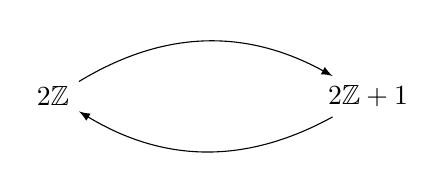
\begin{tikzpicture}[node distance=2cm, main/.style = {}]
	\tikzset{edge/.style = {->,> = latex}}
	
		\node[main] (1) [] {};
		\node[main] (2) [left of=1] {$ 2\mathbb{Z} $};
		\node[main] (3) [right of=1] {$ 2\mathbb{Z} + 1 $};
		
		\draw[edge] (2) to[bend left] (3);
		\draw[edge] (3) to[bend left] (2);
	\end{tikzpicture}
\end{center}

In generale, una classe di equivalenza $ C $ con periodo $ q > 1 $ può essere suddivisa in q sottoinsiemi:
$$ C = C_0 \dot\cup C_1 \dot\cup ... \dot\cup C_{q-1} $$

\begin{center}	
	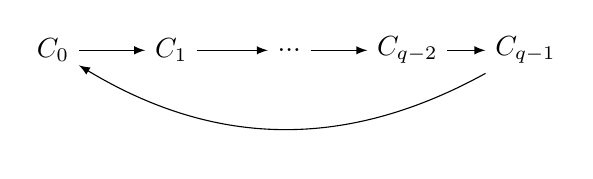
\begin{tikzpicture}[node distance=1.5cm, main/.style = {}, edge/.style = {->,> = latex}]

	
	\node[main] (1) [] {$ C_0 $};
	\node[main] (2) [right of=1] {$ C_1 $};
	\node[main] (3) [right of=2] {$ ... $};
	\node[main] (4) [right of=3] {$ C_{q-2} $};
	\node[main] (5) [right of=4] {$ C_{q-1} $};
	
	\path[edge]
	(1) edge node[] {} (2)
	(2) edge node[] {} (3)
	(3) edge node[] {} (4)
	(4) edge node[] {} (5)

	(5) edge[bend left] node[] {} (1);

	\end{tikzpicture}
\end{center}

E la catena di Markov percorre in maniera ciclica le classi. 

%TODO hai perso l'inizio

$ s $ è uno stato \textbf{ricorrente} se $ f_s $ = 1 (torniamo almeno una volta - in realtà infinite);

$ s $ è uno stato \textbf{transiente} se $ f_s < 1 $.

La probabilità di tornare infinite volte in uno stato ricorrente è 1. La probabilità di tornare almeno 2 volte in uno transiente è $ f_s^2 $; la probabilità di tornare almeno $ n $ volte è $ f_s^n $.

Negli stati transienti, %TODO assumo siano gli stati transienti quelli di cui stiamo parlando ora
la probabilità di tornare infinite volte invece è 0. La catena di Markov passa per gli stati transienti con probabilità 1 un numero finito di volte. 

\paragraph{Esempio: passeggiata aleatoria simmetrica}

La probabilità di tornare a 0 dopo $ 2n $ passi, oppure la probabilità che la passeggiata sia diversa da 0 per $ 2n $ passi si indica con la stessa quantità:

$$ P(x_{2n} \ne 0, x_{2n-1} \ne 0, ..., x_{1} \ne 0 | x_0 = 0) = u_{2n} = \binom{2n}{n}\frac{1}{2^{2n}}$$

$$u_{2n} \overset{ \text{per Stirling} }{\simeq} \frac{1}{\sqrt{\pi n}} \underset{n \to \infty}{\longrightarrow} 0$$

0 quindi è uno stato ricorrente per la passeggiata aleatoria simmetrica. 

Ad esempio, se consideriamo i soliti due giocatori che usano una moneta simmetrica, la probabilità che il guadagno non arrivi mai al pareggio è pari a 0. 

\subsection{Verificare se uno stato è transiente o ricorrente}
C'è una proprietà che semplifica il verificare se uno stato è transiente o ricorrente:

$ s $ è ricorrente se e solo se:
$$ \sum_{n=0}^{\infty} p_{s,s}^{n} = \infty $$
$ s $ è transiente se e solo se:
$$ \sum_{n=0}^{\infty} p_{s,s}^{n} < \infty \qquad \text{(la serie è convergente) } $$

\paragraph{Esempio} Applichiamo il metodo appena esposto considerando per esempio una passeggiata aleatoria su $ \mathbb{Z} $.
$$ p = \frac{1}{2} \qquad p_{0,0}^{(2n)} = u_{2n} = \binom{2n}{n}\frac{1}{2^{2n}} \simeq \frac{1}{\sqrt{\pi n}} $$

$$ \sum_{n=0}^{\infty} p_{0,0}^{(n)} = +\infty $$
Dobbiamo considerare la serie $\frac{1}{\sqrt{n}}$ che è divergente per $ n \ge \frac{1}{2} $ e converge per $ n < \frac{1}{2} $. In questo caso è divergente. 

$$ p \ne \frac{1}{2} \qquad p_{0,0}^{(2n)} = \binom{2n}{n} p^n (1-p)^n = \underbrace{\binom{2n}{n}\frac{1}{2^2n}}_{\displaystyle = u_{2n} \simeq \frac{1}{\sqrt{\pi n}}} \cdot \; \underbrace{2^{2n} p^n(1-p^n) }_{\displaystyle = 4p(1-p^n)} $$

Consideriamo la funzione $ p(1-p) $:

$$ \frac{\partial}{\partial{p}} p(1-p) = 1.p -p = 1 - 2p $$
È positiva per $ p < \frac{1}{2} $ e negativa per $ p > \frac{1}{2} $.

\begin{multicols}{2}
	\begin{tikzpicture}
		\begin{axis}[axis lines=left, xtick={0,1}, ytick={0.25}, ymax=0.3, xmax=1.1, width=7cm]
			\addplot [
			domain=0:1, 
			samples=100, 
			color=black,
			]
			{x*(1-x)};
		\end{axis}
	\end{tikzpicture}
	
	Questa quantità: $ (4p(1-p))^n $ è sempre minore di 1. È una serie geometrica convergente; allora, in questo caso lo stato 0 è transiente. 
\end{multicols}

I due giocatori andranno in pareggio solo un numero finito di volte. 

%TODO che cavolo è la roba sotto

\begin{align*}
	& f_{s,s}^{(0)} \\
	U(z) & = \sum_{n=0}^{\infty} p_{s,s}^{(n)} z^n \\
	& |z| < 1 \\
	F(z) & = \sum_{n=1}^{\infty} f_{s,s}^{(n)} z^n
\end{align*}

Osserviamo che $ U(z) = 1 + F(z)\cdot U(z) $. Si vede dall'equazione del rinnovamento. 

La probabilità di tornare a $ s $ dopo $ n $ passi è:
$$ p_{s,s}^{(n)} = \sum_{k=1}^{n} f_{s,s}^{(k)} p_{s,s}^{(n-k)} \qquad \text{con } n \ge 1 $$
C'è quindi una prima volta dove arriviamo a $ s $ ($ f_{s,s}^{(k)} $) e poi ci torniamo una seconda volta (al tempo $ n-k $). 

Per Markov è come se la catena ripartisse dall'inizio. 


 $$ U(z) = \sum_{n=0}^{\infty} p_{s,s}^{(n)} z^n $$
 
Per $ n = 0, p_{s,s}^0 = 1 $ quindi 

$$ U(z)	= 1 + \sum_{n=1}^{n} (\sum_{k=1}^{n} f_{s,s}^{(k)} p_{s,s}^{(n-k)}) z^n $$

Introduciamo $ m = n-k \Rightarrow n=m+k $

\begin{align*}
	U(z) & = 1 + \sum_{m=0}^{\infty} \sum_{k=1}^{\infty} f_{s,s}^{(k)} p_{s,s}^{(m)} \equalto{z^{m+k}}{z^m\cdot z^k} \\
	& = 1 + (\sum_{m=0}^{\infty}p_{s,s}^{(m)} z^m )(\sum_{k=1}^{\infty} f_{s,s}^{(k)}z^k ) \\
	& = 1 + F(z)\cdot U(z) \\
	\lim\limits_{z \uparrow 1} \sum_{n=1}^{\infty} f_{s,s}^{(n)} z^n & = \sum_{n=1}^{\infty} f_{s,s}^{(n)} = f_s \\
	\lim\limits_{z \uparrow 1} U(z) & = \sum_{n=0}^{\infty} p_{s,s}^{(n)} \\
	U(z) & = \frac{1}{1 - F(z)}
\end{align*}

Nel caso del periodo abbiamo che due stati con la stessa classe di equivalenza hanno lo stesso periodo. Anche la ricorrenza/transienza hanno la stessa proprietà (ovvero, due classi di equivalenza hanno la stessa ricorrenza/transienza). 

\paragraph{Lemma} Dato uno stato $ s $ ricorrente, se $ s \prec s' $ allora $ s' \prec s $.

Supponiamo per assurdo $ s' \nprec s $.

$ \exists n_1 : p_{s,s'}^{(n_1)} > 0$.

Quindi posso tornare un numero finito di volte su $ s $. Ma se uno stato è ricorrente, posso tornare infinite volte in uno stato. ASSURDO
Quindi $ s' \approx s $

\paragraph{Lemma} Se $ s \approx s' $ e $ s $ è ricorrente, allora $ s' $ è ricorrente. 

Questo lemma ci dice che una classe di equivalenza ha tutti stati ricorrenti, oppure tutti stati transienti. 

Supponiamo $ s $ ricorrente; supponiamo $ s \approx s' $. Quindi $ s \prec s' $ e $ s' \prec s $. 

$$ \Rightarrow \exists n_1 : P_{s,s'}^{(n_1)} > 0 \land \exists n_2 : p_{s,s'}^{(n_2)} > 0 $$

$$ \sum_{n=0}^{\infty} p_{s',s'}^{(n)} \ge \sum_{n = n_1 + n_2}^{\infty} p_{s',s'}^{(n)} $$ 

Se partiamo da $ n = n_1+n_2 $, come facciamo ad andare da $ s' $ a $ s' $? Andiamo in $ n_2 $ da $ s' $ a $ s $, e in ???: %TODO

$$ \ge \sum_{n=n_1+n_2}^{\infty} p_{s',s}^{(n_2)} p_{s,s}^{(n-n_1-n_2)} p_{s,s'}^{(n_1)} $$
Sia $ k = n-n_1-n_2 $:
$$ = p_{s',s}^{n_2} p_{s,s'}^{(n_1)} \sum_{k=0}^{\infty} p_{s,s}^{(k)} = +\infty$$

$$ \Rightarrow s' \text{ è ricorrente.} \qed $$

\section{Teorema ergodico per catene di Markov}
$$ 
\begin{array}{cc}
	s \in S & v_s = \sum_{n=1}^{\infty} n f_{s,s}^{(n)} \text{ (attesa del tempo di ritorno)} \\
	s \text{ ricorrente } & f_s = \sum_{??}^{??} ?? = 1 \\ %TODO 
\end{array} $$

$$ p_{s,s'}^{(n)} \underset{n \to \infty}{\longrightarrow} \frac{1}{v_s} $$
$$ \text{se } v_s = +\infty, \; \; \frac{1}{v_s} = 0 $$

Se $ v_s = +\infty $ allora non è necessario che sia aperiodica. 

Questo teorema (che non dimostreremo) è interessante perché ??? %TODO
Si può vedere che facendo andare avanti la catena di Markov e contando quante volte passa per $ s $, la frequenza/percentuale di tempo tende a questo limite. 

È come nel caso dello schema di Bernoulli; per la legge dei grandi numeri, se contiamo quante volte otteniamo il successo, questa quantità tende alla probabilità. La probabilità ha il significato di frequenza.

Anche nelle catene di Markov che sono dipendenti ??? %TODO

Questo valore è l'attesa del tempo di ritorno; c'è però un metodo più semplice per calcolarlo. 

Supponiamo nel caso finito che uno stato sia ricorrente, ci sia una sola classe di di equivalenza (e quindi tutti gli stati sono ricorrenti) e aperiodici. 
\\ \\
Sappiamo che $ p_{s',s}^{(n)} \to v_s^{-1} = u_s $.
\\ \\
Osservazione: $ p_{s',s}^{(n+1)} = \sum_{s''} p_{s',s''}^{(n)} p_{s'',s} $

$$ \begin{array}{cc}
	p_{s,s'}^{(n+1)} \underset{n \to \infty}{u_s} & \sum_{s''}p_{s',s''}^{(n)} p_{s'',s} \\ 
	%TODO
	u_s = \sum_{s''} ??? & \sum_{s \in S} u_s = 1
\end{array} $$

$ u_s $ è una distribuzione di probabilità sugli stati;

$$ \sum_{s \in S} p_{s'', s}^{(n)} = 1 \qquad \forall s \in S $$

$$ u_s = \sum_{s''} u_{s''}p_{s'',s}$$

Ho un sistema di equazioni lineari: abbiamo $ k $ incognite (gli stati) e $ k+1 $ equazioni. Ma le equazioni $ \sum_{s''} p_{s'', s}  \forall s \in S$ non sono linearmente indipendenti, quindi ne posso prendere solo una. Il mio sistema diventa:

$$ 
\begin{cases} \sum u_s = 1 \\ u_s = \sum_{s''} u_{s''}p_{s'',s} \forall s \in S \end{cases} 
$$

Supponiamo ora:

$$ \sum_{s \in S} v_s = 1 \qquad \qquad \qquad v_s = \sum_{s''} v_{s''}p_{s'',s} $$

Con $ S $ finito. C'è un'unica soluzione:

\begin{align*}
	v_s & = \sum_{s''}v_{s''}p_{s'',s}^{(n)} \\
	& = \sum_{s''}v_{s''}u_s = u_s ??? %TODO
\end{align*}
\vspace{1cm}
\hrule  %TODO riguarda inizio
\vspace{1cm}
Definiamo ora $ \mu_s = \sum_{n=1}^{\infty} n \cdot f_s^{(n)} $

Allora $ p_{s,s'}^{(n)} \to \ddfrac{1}{\mu_s} $

Quindi è uguale a 0 se $ \mu = +\infty $. Se $ \mu= +\infty $, non è necessaria aperiodicità. 

Nel caso $ S $ finito, $ u_s = \ddfrac{1}{\mu_s} \qquad \displaystyle \sum_{s \in S} \mu_s = 1 $ %TODO controlla sua \mu_s nella sommatoria

$$ \forall s' \qquad \sum_{s} u_s p_{s,s'} = u_s'$$

Queste relazioni ci dicono che $ u_s $ è una distribuzione invariante o stazionaria, ovvero se mettiamo $ u_s $ come stato iniziale in una catena di Markov, vediamo che nei tempi successivi ??? %TODO

Vogliamo verificare se la proprietà sia vera anche nel caso $ S $ infinito. 

Dato $ \bar{s} \in S $,

$$ p_{\bar{s},s'}^{(n+1)} = \sum_{s \in S} p_{\bar{s}, s}^{(n)} p_{s,s'} $$


Questa è una serie, dobbiamo passare al limite. Nel caso infinito però non è sempre vero che il limite della serie è uguale alla serie dei limiti. Consideriamo $ \bar{S} \subset S $ finito anziché $ S $:

\begin{align*}
	p_{\bar{s}, s'}^{(n+1)} & \ge \sum_{s \in \bar{S} } p_{\bar{s},s}^{(n)} p_{s,s'} \qquad \text { per il teorema ergodico} \\
	u_{s'} & \ge \sum_{s \in \bar{S}} u_s p_{s,s'} \\
	u_{s'} & \ge \sum_{s \in S} u_sp_{s,s'} \qquad \text{(I)}
\end{align*}

Abbiamo dimostrato una disuguaglianza. Definiamo 
$$ 0 < \alpha = \sum_{s \in S} u_s \le 1 \qquad \text{(II)} $$
$\alpha > 0$ perché gli $ u_s > 0$, ma $ \alpha \le 1$ perché $ \sum_{s' \in S} p_{s,s'}^{(n)} = 1 $

Dobbiamo dimostrare che in (I) c'è uguaglianza, e in (II) che la somma è pari a 1.

Supponiamo per assurdo che non ci sia uguaglianza in (I) per un particolare stato $\bar{s}'$:

$$ u_{\bar{s}'} > \sum_{s \in S} u_s p{s,s'} $$

Allora quando sommiamo tutti gli stati, avremo la disuguaglianza stretta:
$$ \sum_{s'} u_{s'} > \sum_{s'} \sum_{s} u_s p_{s,s'} $$
$$ \alpha = \sum_{s'} u_{s'} > \sum_{s'} \sum{s} u_s p_{s,s'}$$
$$ \alpha > \alpha \text{ ASSURDO } $$

Quindi anche nel caso infinito, $ u_s $ è una distribuzione di probabilità, cioè la somma è pari a 1:

\begin{align*}
	u_{s'} & = \sum_{s} u_s p_{s,s'}^{(2)} \\
	u_{s'} = \sum_{s} u_s p_{s,s'} ^{(n)}
\end{align*}

Per $ n \to \infty $, $ u_{s'} = \sum_{s} u_su_{s'}$
\begin{align*}
u_{s'} & = \alpha u_{s'} \qquad \qquad u_{s'} > 0 \\
& \Rightarrow \alpha = 1 \qed
\end{align*}

Abbiamo ipotizzato finora l'attesa di ritorno $\mu_s < +\infty$ (cioè $\mu_s$ finito).

Nel caso $\mu_s = + \infty$, allora $ p_{s,s'} \to 0 $. Lo abbiamo visto nel caso aperiodico, ma questa proprietà è vera anche nel caso generale. Questo ci porta a fare una classificazione degli stati ricorrenti in 2 categorie:

$$ \text{supponiamo } s \text{ ricorrente: } \begin{cases*}
	\mu_s < +\infty, & s \text{ ricorrente positivo} \\
	\mu_s = + \infty, & s \text{ricorrente nullo}
\end{cases*}$$

Nel primo caso quindi l'attesa del tempo di ritorno è finita, nel secondo infinita. 
\\
\\
Supponiamo di avere una classe di equivalenza $ S $ irriducibile e ricorrente. Vogliamo mostrare che non è possibile che ci sia uno stato ricorrente positivo e uno stato ricorrente nullo. Supponendo quindi che $ s_1 $ sia positivo, vogliamo mostrare che $ s_2 $ non può essere ricorrente nullo. 

Dato un $ s $,
$$ p_{s,s{_1}}^{(n)} \underset{n \to \infty}{\longrightarrow} u_{s_{1}} > 0$$

$$ \exists n_1 : p_{s_1, s_2}^{n_1} > 0 \qquad \text{perché } s_1, s_2 \in S  $$

Ma $ p_{s,s_2}^{(n)} > p_{s,s_1}^{(n - n_1)} p_{s,s_2}^{(n_1)} $

$ p_{s,s_2}^{(n)} $ non tende a 0 (per $ n \to \infty $)

$$ \Rightarrow s_2 \text{ è ricorrente positivo} \qed $$

Una conseguenza è che se $ S $ è finito, non ci sono stati ricorrenti nulli, perché 

\formule{\sum_{s' \in S} p_{s,s'}^{(n)} = 1}{essendo S finito, possiamo passare al limite della somma. Se gli stati fossero ricorrenti nulli, il limite tenderebbe a 0, ma non è possibile.}

??? %TODO riguarda lezione

Vediamo il caso più semplice di catena di Markov con spazio degli stati finiti, che è una catena di Markov con due stati: $ S = \{0,1\} $. La matrice di transizione è: %TODO si chiama così?

$$ \Pi = \left(\begin{matrix}
	p & 1-p \\
	1-q & q
	\end{matrix}\right)  \qquad \qquad 
	\begin{array}{c} 
		0 < p < 1 \\ 
		0 < q < 1 
	\end{array}
$$

\begin{enumerate}
	\item $ u_0 + u_1 = 1 \qquad \qquad $ (perché è una distribuzione di probabilità)
	\item $u_0 \cdot p + u_1 \cdot (1-q) = u_0 $
	\item $u_1 \cdot q + u_0 \cdot (1-p) = u_1 $
\end{enumerate}

2. e 3. sono uguali, possiamo usare 1. e 2. 
$$ \begin{cases*}
	u_0 = u_1\left(\ddfrac{1-q}{1-p}\right) \\
	u_1\ddfrac{1-q}{1-p} + u_1 = 1
\end{cases*}$$
$$  
	\begin{cases*}
		u_1 \ddfrac{(1-q)+(1+p)}{1-p} = 1 \\
		u_0 = u_1(\ddfrac{1-q}{1-p})
	\end{cases*}
	\qquad 
	\begin{cases*}
		u_0 = \ddfrac{1-q}{2-p-q} \\
		u_1 = \ddfrac{1-p}{2-p-q} 
	\end{cases*}
$$

Possiamo rappresentare la passeggiata aleatoria con un cerchio:

\begin{center}
	\begin{tikzpicture}[point/.style={inner sep=2pt, fill=black, circle}]
		%\draw[red, thick] (0,0) circle (2 cm);
		
		\node[point, label=0] (1) at (0,2) {};	
		\node[point, label=1] (2) at (1.5,1.5) {};	
		\node[point, label=2] (3) at (2,0) {};	
		\node[point, label=3] (4) at (1.3,-1.7) {};	
		\node[point, label=4] (5) at (-1.3,-1.7) {};	
		\node[point, label=...] (6) at (-2,0) {};	
		\node[point, label=$ r-1 $] (7) at (-1.5,1.5) {};	
		
		\path []
		(1) edge[bend left, ->] (2)
		(1) edge[bend right, ->] (7); 
		
		\node[] (8) at (6,1) {$ |S| = n $};
		
	\end{tikzpicture}	
\end{center}

Se $ r $ è dispari, è aperiodica. %TODO che cosa? la passeggiata?

\begin{align*}
	& u_0 + u_1 + ... + u_{r-1} = 1 \\
	& 1 \le s \le r-2 \\
	u_s & = u_{s-1} p + u_{s+1}(1-p) \\
	u_0 & = u_{r-1}p + u_1(1-p) \\
	u_{r-1} & = u_{r-2} p + u_0(1-p)
\end{align*}

Abbiamo $ r+1 $ equazioni e $ r $ incognite. Ipotizziamo che $ u_s = \frac{1}{r} $.

Questa è in realtà una distribuzione invariante anche nel caso pari, ma nel caso pari non è periodico. 


???%TODO


In entrambi i modelli di \textbf{Laplace-Bernoulli} e \textbf{Ehrenfest} abbiamo due urne. Nel primo scegliamo a caso una pallina e la spostiamo da un'urna all'altra; nel secondo, abbiamo $ n $ palline bianche e $ n $ palline nere. Di queste $ 2n $ palline, metà stanno nell'urna A e metà nell'urna B. Possiamo prendere come stato il numero delle palline bianche in A. Quello che osserviamo è che il modello di Ehrenfest non è aperiodico. 

???%TODO

Nel modello di Laplace-Bernoulli il numero di palline bianche può anche rimanere invariato:

\begin{center}
	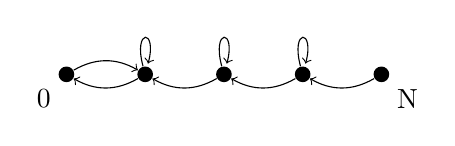
\begin{tikzpicture}[point/.style={circle, inner sep=2pt, fill=black}]
		\node[point, label=below left:0] (0) at (-2,0) {};
		\node[point] (1) at (-1,0) {};
		\node[point] (2) at (0,0) {};
		\node[point] (3) at (1,0) {};
		\node[point, label=below right:N] (4) at (2,0) {};
		
		\path[e/.style={bend left, ->}]
		(0) edge[e] (1)
		(1) edge[e] (0)
			edge[loop above] (1)
		(2) edge[e] (1)
			edge[loop above] (2)
		(3) edge[e] (2)
			edge[loop above] (3)
		(4)	edge[e]	(3);
		
	\end{tikzpicture}
\end{center}

se scambiamo 2 palline bianche tra le urne A e B, il numero delle palline bianche in A è invariato. Se la probabilità di rimanere nello stato è 0, allora il periodo deve essere 1  e possiamo usare il teorema ergodico. Intuitivamente, comunque, possiamo affermare che 

$$ u_s < \frac{\binom{N}{S}\binom{N}{N-S}}{\binom{2N}{N}} $$

e questa disuguaglianza dovrà soddisfare le equazioni. 

\paragraph{Teorema} Supponiamo S infinito, una sola classe di equivalenza aperiodica irriducibile. Supponiamo ci sia una distribuzione invariante $ u_s $, con $ 0 \le u_s \le 1 $:
$$ \sum_{s}u_s = 1 \qquad \forall s', u_{s'} = \sum_{s} u_s p_{s,s'} $$
Allora gli stati sono ricorrenti positivi. 
\\
\\
Dobbiamo far vedere che non sono ricorrenti nulli o transienti. Supponiamo per assurdo siano transienti:
$$ ??? \; \sum_{n} p_{s,s^*}^{(n)} < +\infty $$ %TODO
Se prendiamo $ s' \ne s $, 
$$ p_{s',s^*}^{(n)}\underset{n\to 0}{\longrightarrow} 0$$
Possiamo scrivere l'equazione del rinnovamento:
$$ p_{s',s}^{(n)} \sum ???$$ %TODO
??? %TODO

\section{Modello di coda}
In questo modello abbiamo dei clienti, che arrivano e vanno dagli sportelli dove vengono serviti. Il tempo che passano agli sportelli è aleatorio. Supponiamo che il tempo sia discreto. 

Uno sportello può contenere un cliente, gli altri clienti sono in coda. 

Definiamo $ p $ la \textbf{probabilità di arrivo di un cliente}, mentre $ q $ la probabilità di \textbf{fine del servizio}. Gli arrivi dei clienti e la fine del servizio sono indipendenti. 

Questo è descritto da una catena di Markov in cui lo spazio degli stati è $ \mathbb{N} $: $ S = \mathbb{N} = \{0, 1, ...\} $.

Ci chiediamo ora qual è la probabilità, partendo da 0, di rimanere nello stato 0 (ovvero che non ci sia nessun cliente e che non arrivi nessun cliente), e altre probabilità:
$$ \begin{array}{ccc}
  p_{0,0} = 1-p & p_{1,1} = p\cdot q + (1-p) 1-q  & p_{1,2} = p(1-q) \\
  p_{0,1} = p & p_{1,0} = (1-p)q & 
\end{array} $$

$ p_{1,1} $ indica la probabilità che, dopo aver finito di servire un cliente ne arrivi uno nuovo; oppure di non finire di servire un cliente, e che non arrivi nessun nuovo cliente. 

In generale, per $ s \ge 1 $:
\begin{align*}
	p_{s,s} & = p\cdot q + (1-p) (1-q) & = r \\
	p_{s,s-1} & = (1-p)q & = l \\
	p_{s,s+1} & = p(1-q) & = d
\end{align*}

Questa passeggiata è ricorrente positiva? Se esiste una distribuzione invariante si, se non esiste o gli stati sono ricorrenti nulli oppure transienti. 

Definiamo $ u_i $, con $ i \in \mathbb{N} $:
\begin{align*}
	\sum_{i=0}^{\infty} u_i & = i \\
	u_0 & = u_0(1-p) + u_1 l \\
	u_1 & = u_0 p + u_1 r + u_r l \\
	u_s & = u_{s-1}d + u_s r + u_{s+1} l, \qquad \qquad s \ge 2 \\
	u_1 l & = u_0 p \\
	u_1(1-r-l) & = u_2 l \\
	u_1 d & = u_2 l \\	
	u_s d = u_{s+1} l
\end{align*}

Mettiamo insieme le equazioni:
$$ u_1 = u_0 \frac{p}{l} \qquad \qquad u_2 = u_1\frac{d}{l} \qquad \qquad u_{s+1} = u_s \frac{d}{l} $$
Riscritte in termini di $ u_0 $:
$$ u_2 = u_0 \frac{p}{l}\frac{d}{l} \qquad \qquad u_s = u_0 \frac{p}{l} \left(\frac{d}{l}\right)^{s-1} $$

Sapendo che $ \sum_{i=0}^{\infty} u_i = 1 $:

$$ u_0 \left( 1 + \frac{p}{l} + \frac{p}{l}\frac{d}{l} + \frac{p}{l} \left(\frac{d}{l}\right)^2 + ... \right) = 1 $$

L'equazione è possibile solo se questa serie:
$$ u_0 \left(1 + \frac{p}{l} \left( \sum_{j=0}^{\infty} \left(\frac{d}{l}\right)^j\right)\right) $$

è convergente; ma questa è una serie geometrica, ed è convergente per $ \frac{d}{l} = 1 $.

$$ \begin{array}{cc}
d = p(1-q) & l = q(1-p) \\
p(1-q) < q(1-p) & ??? \\ %TODO
\frac{p}{1-p} < \frac{q}{1-q} & p < q
\end{array} $$

Intuitivamente, $ p $ è la probabilità di arrivo di un cliente, $ q $ la probabilità che un cliente vada via. ???? %TODO

Questo fa sì che non si formi una coda lunga. Se $ p < q $, allora abbiamo che gli stati sono \textbf{ricorrenti positivi}. Se $ p \ge q $, gli stati sono \textbf{ricorrenti nulli} oppure \textbf{transienti}. 

Ci possiamo ricondurre al problema della rovina del giocatore: in quel caso è una passeggiata aleatoria in cui possiamo aumentare o diminuire di 1. Qui però c'è anche la possibilità di rimanere nello stesso stato all'istante successivo. Ma se trascuriamo questi tempi, nel caso $ p = q $, $ \Rightarrow \frac{p}{1-p} = \frac{q}{1-q} $, siccome le probabilità di andare a destra e a sinistra sono uguali, il modello corrisponde alla passeggiata simmetrica. 






















\backmatter
% bibliography, glossary and index would go here.



\end{document}